\chapter{人工智能的应用、挑战与未来展望}

本章将从宏观层面探讨人工智能对社会各领域的影响,并分析其带来的挑战和未来的发展方向。

\section{AI的广泛应用}

人工智能的涟漪已然荡开,浸润着社会肌理的每一寸,如春风化雨般,悄然间催生出生产力的新芽,亦为寻常巷陌注入了便捷的甘泉。

我们正站在一个由人工智能重塑的时代门槛上,它不仅是冰冷的算法和代码,更是赋能人类潜能的强大工具。在医疗健康领域,AI正成为医生的“第三只眼”,精准诊断疾病,加速新药研发,为生命健康构筑起一道坚实防线。它不再仅仅是辅助工具,而是深度参与到疾病的早期筛查、个性化治疗方案的制定中,让医学的边界不断拓展。

在金融的世界里,AI如一位敏锐的风险管家,洞察着市场的瞬息万变,识别潜在的欺诈行为,守护着我们的财富安全。它在海量数据中抽丝剥茧,提前预警风险,让金融交易更加透明、公正。交通领域,从自动驾驶的未来愿景,到智能物流的实时优化,AI正在重新定义出行的效率与安全,让货物运输更智慧,人们的旅途更便捷。而工业的脉搏,也因AI而强劲跳动,智能制造让生产线拥有了“大脑”,预测性维护则让机器的“生命”得以延长,极大提升了生产效率和产品质量。在教育的天空下,AI如一位耐心且智慧的导师,为每一个学生量身定制学习路径,让知识的获取变得更高效、更个性化,真正实现因材施教。

不仅在产业深处,AI也以润物细无声的方式渗透进我们的日常生活。智能家居让我们的居所变得更懂我们,一句话便能掌控光影与温度,营造出舒适温馨的港湾。个性化推荐算法如同贴心的向导,在浩瀚的信息海洋中精准捕捉我们的喜好,无论是电影、音乐还是商品,总能恰到好处地呈现在眼前。而那些无处不在的智能助手,无论是手机里的语音伙伴,还是在线客服,都让信息触手可及,让生活琐事变得更加从容不迫。

人工智能的崛起,正以前所未有的深度和广度,改变着我们工作、学习和生活的方式,描绘出一幅充满无限可能的新画卷。它不仅仅是技术的迭代,更是人类文明迈向新纪元的关键一步。


\subsection{产业应用}

\begin{itemize}
    \item \textbf{医疗健康:} AI在疾病诊断方面展现出强大的能力,例如通过影像识别辅助医生发现早期病变;在药物研发领域,AI加速了新药筛选和靶点识别的进程,大幅缩短了研发周期;在临床决策方面,AI通过分析数据优化治疗路径,提升医疗质量。

    \subsubsection{AI赋能疾病的“慧眼”:影像识别的精准诊断}
    在现代医学的诊断过程中,医学影像扮演着至关重要的角色,而人工智能的介入,则赋予了这些影像更深层的解读能力。AI在\textbf{影像识别}方面的强大能力,使得医生能够更早、更准确地发现疾病的细微征兆。这背后,是\textbf{深度学习}(Deep Learning)尤其是\textbf{卷积神经网络}(Convolutional Neural Networks, \textbf{CNNs})等前沿技术的支撑。

    CNNs在处理图像数据方面具有天然的优势,它们通过模拟人脑视觉皮层的分层处理机制,能够自动从海量的医学影像(如CT、MRI、X光、超声等)中学习并提取复杂的特征。例如,在一个典型的医疗影像诊断流程中,AI系统会经过以下步骤:
    \begin{enumerate}
        \item \textbf{数据预处理:} 对原始影像进行去噪、增强、标准化等操作,以提高图像质量。
        \item \textbf{特征提取:} CNNs的多层结构自动学习并提取影像中的局部和全局特征,例如肿瘤的边缘、纹理、密度变化等。
        \item \textbf{模式识别与分类:} 基于提取的特征,AI模型判断影像中是否存在病变,并对其进行分类。
    \end{enumerate}

    \textbf{案例:早期癌症筛查}

    在癌症的早期诊断中,AI影像识别已经取得了显著进展。例如,浙江省肿瘤医院的研究团队利用AI成功从平扫CT中识别早期胃癌。他们通过一个名为“DAMO GRAPE”的模型,对数万例CT影像进行训练,使其能够精准识别早期胃癌病灶。在一个实际案例中,一名患者6个月前的CT片在当时未报告病变,但经过AI模型分析后,却提示存在早期胃癌,这为患者赢得了宝贵的早期治疗时间。

    \subsubsection{AI加速药物研发:从浩瀚分子到精准靶点}
    新药研发是一个漫长、昂贵且高风险的过程。传统上,从靶点发现到药物上市可能需要十年甚至更长时间,耗费数十亿美元。而\textbf{人工智能}的引入,正像一台强大的“加速器”,颠覆着这一传统模式,尤其在\textbf{新药筛选}和\textbf{靶点识别}方面展现出革命性潜力。

    AI在药物研发中的核心技术包括:
    \begin{itemize}
        \item \textbf{机器学习/深度学习模型:} 如\textbf{图神经网络}(Graph Neural Networks, \textbf{GNNs})、\textbf{生成对抗网络}(Generative Adversarial Networks, \textbf{GANs})、\textbf{变分自编码器}(Variational Autoencoders, \textbf{VAEs})等。
        \item \textbf{计算化学与生物信息学:} 结合分子动力学模拟、量子化学计算、蛋白质结构预测等。
    \end{itemize}

    \textbf{原理与应用:}

    \begin{enumerate}
        \item \textbf{靶点识别与验证:} AI可以通过分析海量的基因组学、蛋白质组学、代谢组学等多组学数据,以及医学文献和专利信息,来识别与疾病发生发展密切相关的潜在生物大分子(即药物靶点)。例如,\textbf{知识图谱}结合\textbf{自然语言处理}(NLP)技术,能够从海量非结构化文本中提取信息,构建基因、疾病、化合物和生物通路之间的复杂关系网络,从而快速定位新的靶点。

        $$
        P(\text{Target} | \text{Data}) \propto P(\text{Data} | \text{Target}) \times P(\text{Target})
        $$
        其中,$P(\text{Target} | \text{Data})$表示在给定数据下靶点存在的概率,$P(\text{Data} | \text{Target})$表示给定靶点下数据出现的概率,$P(\text{Target})$是靶点的先验概率。AI通过迭代优化这个概率模型来识别最有潜力的靶点。

        \textbf{案例:Insilico Medicine的靶点发现平台}
        Insilico Medicine公司利用其基于Transformer的知识图谱功能,从全球期刊文献中提取信息,关联基因、疾病、化合物和生物通路,并结合大型语言模型进行问答,以快速识别疾病发展的遗传基础和分子机制,从而加速药物靶点和生物标志物的识别。有案例显示,AI驱动的多组学整合将乳腺癌研究中的靶点发现周期从传统的1-2年缩短至3-6个月。

        \item \textbf{新药筛选与分子设计:} AI可以在庞大的化合物库中进行\textbf{虚拟筛选},预测化合物与靶点之间的结合能力和活性,从而快速筛选出最有潜力的候选分子。同时,\textbf{生成式AI模型}(如GANs和VAEs)能够从头设计具有特定药理活性的新型分子结构,突破传统化学合成的局限性。

        \textbf{案例:抗生素发现与CDK20抑制剂}
        2023年底,《自然》杂志报道了科学家运用AI技术首次发现对耐甲氧西林金黄色葡萄球菌(MRSA)有效的新抗生素,解决了困扰业界60年的难题。AI通过训练模型评估3.9万种化合物的抗菌活性,再利用深度学习模型筛选出对人体安全的化合物。

        在靶向药物开发中,AI也展现了惊人的速度。例如,针对\textbf{CDK20}靶点,一家公司利用AI从靶点识别到获得活性化合物仅用30天,并合成7个分子后就获得了纳摩尔级别的抑制剂。这与传统方法通常需要6-12个月甚至更长时间形成鲜明对比。
    \end{enumerate}

    \subsubsection{AI优化临床决策与治疗路径}
    除了在诊断和研发前端发力,人工智能在优化临床治疗路径、辅助医生进行复杂决策方面也扮演着日益重要的角色。通过分析海量的临床数据,包括电子病历、临床试验结果和治疗指南,AI能够构建精准的预测模型,为患者推荐个性化的最优治疗方案。

    \textbf{案例:基于临床数据的治疗方案比选}

    以接受维生素K拮抗剂(VKA)治疗的髋部骨折患者为例,临床医生面临着如何在术前快速、安全地逆转抗凝效应的决策。这通常涉及到在凝血酶原复合物浓缩物(PCC)、维生素K或常规处理之间做出选择。AI可以通过分析过往的临床试验数据来辅助这一决策过程。

    一个典型的研究流程可能如图 \ref{fig:clinical_trial_patient_selection} 所示,研究者首先从大量患者中筛选出符合条件的受试者,并将其随机分配至不同治疗组。

    \begin{figure}[htbp]
        \centering
        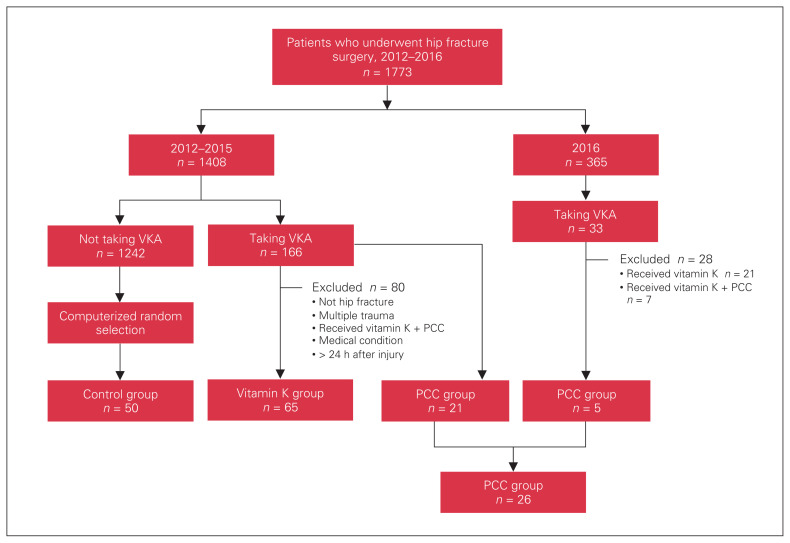
\includegraphics[width=0.7\textwidth]{M2.png}
        \caption{一项关于髋部骨折患者术前抗凝管理的临床研究患者筛选流程图,展示了对照组、维生素K组和PCC组的构成。}
        \label{fig:clinical_trial_patient_selection}
    \end{figure}

    治疗方案本身可以被构建成一个标准化的决策流程,如图 \ref{fig:hip_fracture_treatment_protocol} 所示。这类流程图为开发基于规则或模型的AI临床决策支持系统(CDSS)提供了基础。AI模型可以学习并优化这类流程中的每一个决策节点。

    \begin{figure}[htbp]
        \centering
        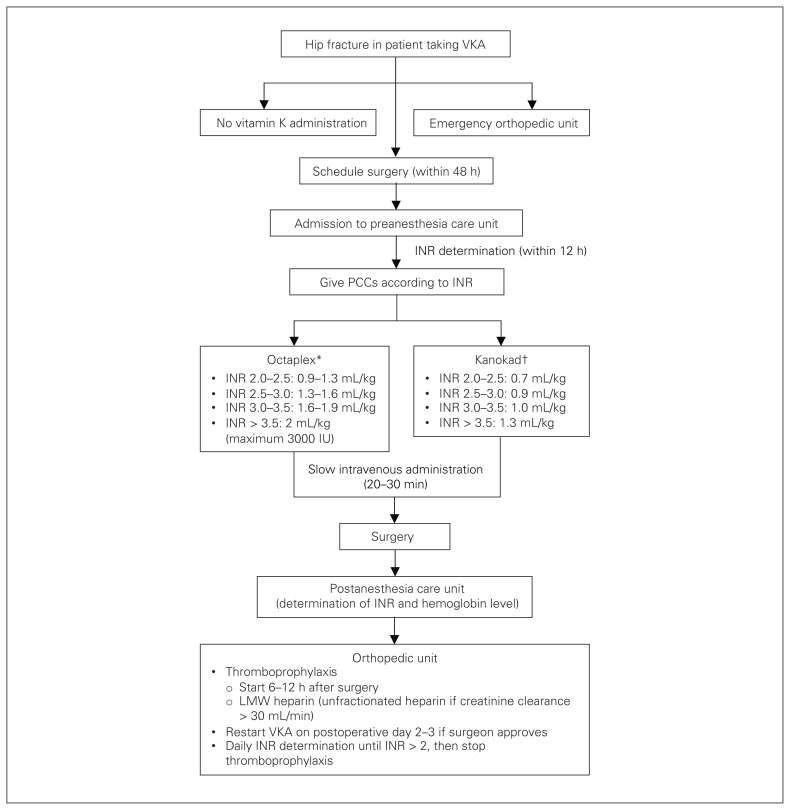
\includegraphics[width=0.8\textwidth]{M1.png}
        \caption{VKA患者髋部骨折围手术期管理流程图,根据术前INR水平决定PCC给药剂量。}
        \label{fig:hip_fracture_treatment_protocol}
    \end{figure}

    AI的核心价值在于,它可以基于实际的临床结果数据,量化不同治疗方案的优劣。例如,通过对不同组别的关键指标——如术前等待时间(time to surgery)和住院时长(length of stay)——进行统计分析(如图 \ref{fig:treatment_outcome_comparison}),AI能够建立预测模型。

    该模型可以被形式化地表达为一个函数 $f$,其目标是预测某个临床结果 $Y$(如住院天数):
    $$
    Y_{pred} = f(X_{\text{patient}}, X_{\text{treatment}}; \theta)
    $$
    其中,$X_{\text{patient}}$ 代表患者的个体特征(如年龄、INR初始值),$X_{\text{treatment}}$ 代表所采取的治疗方案(如PCC、维生素K),$\theta$ 是模型通过学习历史数据得到的参数。AI的目标就是找到最优的 $\theta$,使得预测值 $Y_{pred}$ 与真实结果的误差最小化,从而为新患者推荐能带来最佳预期结果的治疗方案。

    \begin{figure}[htbp]
        \centering
        \begin{subfigure}[b]{0.48\textwidth}
            \centering
            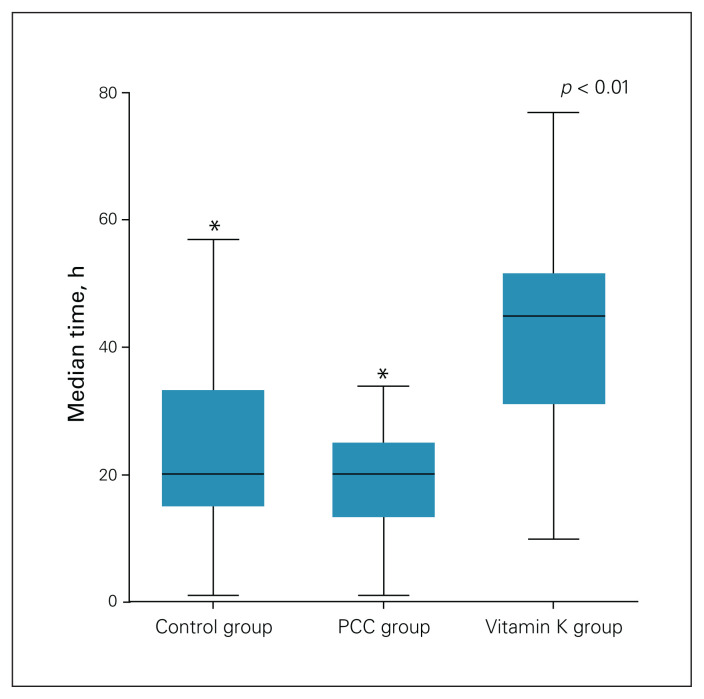
\includegraphics[width=\textwidth]{M3.png}
            \caption{不同治疗方案对中位手术等待时间的影响}
            \label{fig:time_to_surgery_comparison}
        \end{subfigure}
        \hfill
        \begin{subfigure}[b]{0.48\textwidth}
            \centering
            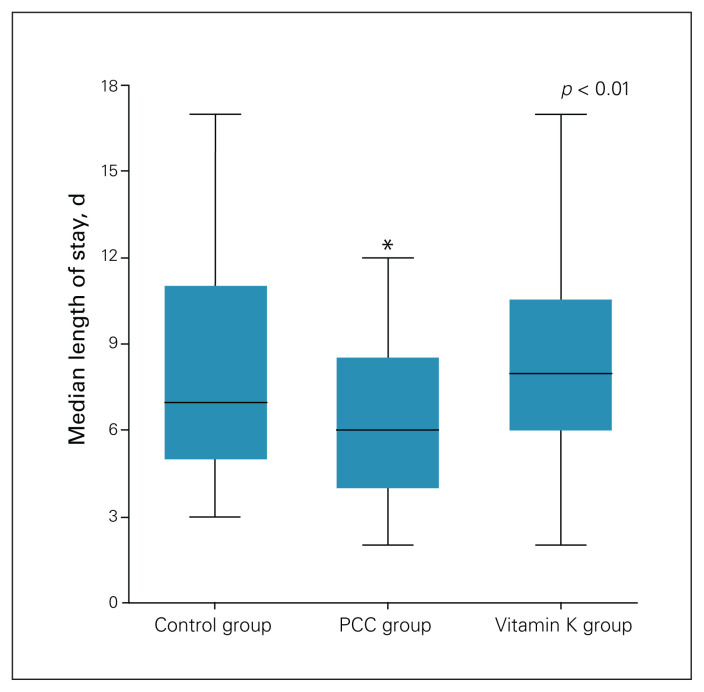
\includegraphics[width=\textwidth]{M4.png}
            \caption{不同治疗方案对中位住院天数的影响}
            \label{fig:length_of_stay_comparison}
        \end{subfigure}
        \caption{PCC组、维生素K组和对照组在关键临床结果上的对比。数据显示,PCC组在缩短手术等待时间和住院天数方面均有显著优势 (p < 0.01),这类数据是训练AI预测模型的宝贵资源。}
        \label{fig:treatment_outcome_comparison}
    \end{figure}

    通过这种方式,AI不仅能够验证现有临床指南的有效性,还能发现更优的、更具个性化的治疗策略,最终提升医疗质量和效率。
    
    \item \textbf{金融:} 人工智能已深度重塑金融行业,其应用贯穿风险管理、欺诈检测、量化交易和财富管理等多个核心领域,通过复杂的算法模型提升决策效率与精准度。

    \subsubsection{AI驱动的智能风险管理与信用评估}
    传统的信用风险评估多依赖于线性模型和有限的结构化数据,而人工智能,特别是\textbf{机器学习}模型,能够整合海量、多维度的数据(包括非传统的另类数据),进行更精准的信用风险定价。
    \begin{itemize}
        \item \textbf{核心技术:} 主要采用\textbf{监督学习}算法,如\textbf{逻辑回归(Logistic Regression)}、\textbf{支持向量机(SVM)}、\textbf{梯度提升决策树(Gradient Boosting Decision Trees, GBDT)}以及\textbf{深度神经网络(DNNs)}。这些模型能够从历史数据中学习复杂的非线性关系,识别出人眼难以发现的风险模式。

        \item \textbf{原理与公式:} 以逻辑回归为例,其目标是预测一个借款人违约的概率。该概率 $P(Y=1 | X)$ 可以通过Sigmoid函数表示:
        $$
        P(Y=1 | X) = \frac{1}{1 + e^{-(\beta_0 + \beta_1 X_1 + \dots + \beta_n X_n)}}
        $$
        其中,$Y=1$ 代表违约事件,$X = (X_1, \dots, X_n)$ 是借款人的特征向量(如收入、负债、信用历史、消费行为等),$\beta = (\beta_0, \dots, \beta_n)$ 是模型通过训练数据学习到的参数。AI模型通过优化算法(如梯度下降法)来找到最佳的 $\beta$ 值,从而最小化预测概率与实际结果之间的误差。
    \end{itemize}

    \subsubsection{基于聚类的客户分群与异常检测}
    理解客户是金融服务的基础。AI通过\textbf{无监督学习}中的\textbf{聚类}技术,能够自动地将具有相似特征或行为模式的客户划分到同一群体,从而实现精准营销和个性化服务。
    \begin{itemize}
        \item \textbf{核心技术:高斯混合模型(Gaussian Mixture Model, GMM)}是一种强大的概率聚类算法。它假设所有数据点来自于一个包含K个高斯分布(如图 \ref{fig:gmm_components_example})的混合模型。与K-Means等硬聚类算法不同,GMM提供“软聚类”,即每个数据点属于各个簇的概率。
        
        \begin{figure}[htbp]
            \centering
            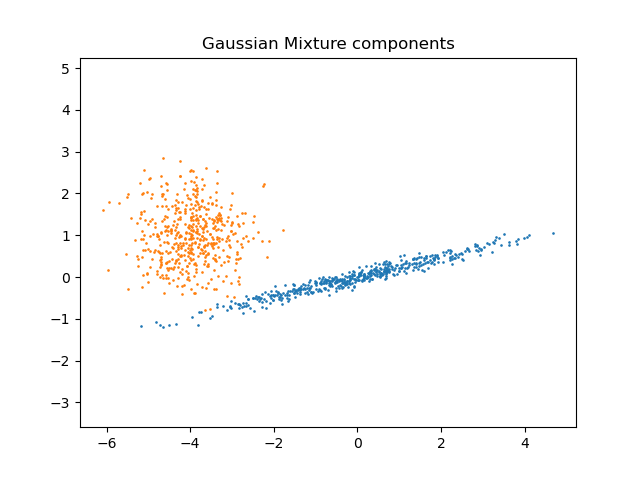
\includegraphics[width=0.6\textwidth]{F7.png}
            \caption{高斯混合模型中两个成分(高斯分布)的散点图示例。}
            \label{fig:gmm_components_example}
        \end{figure}

        \item \textbf{原理与公式:} GMM的概率密度函数定义为:
        $$
        p(x) = \sum_{k=1}^{K} \pi_k \mathcal{N}(x | \mu_k, \Sigma_k)
        $$
        其中,$K$ 是混合成分的数量,$\pi_k$ 是第 $k$ 个高斯分布的混合权重($\sum \pi_k = 1$),而 $\mathcal{N}(x | \mu_k, \Sigma_k)$ 是一个均值为 $\mu_k$、协方差矩阵为 $\Sigma_k$ 的高斯分布。模型通常通过\textbf{期望最大化(Expectation-Maximization, EM)}算法来学习这些参数。如图 \ref{fig:gmm_initialization_comparison} 展示了不同初始化方法对EM算法收敛效果的影响。

        \begin{figure}[htbp]
            \centering
            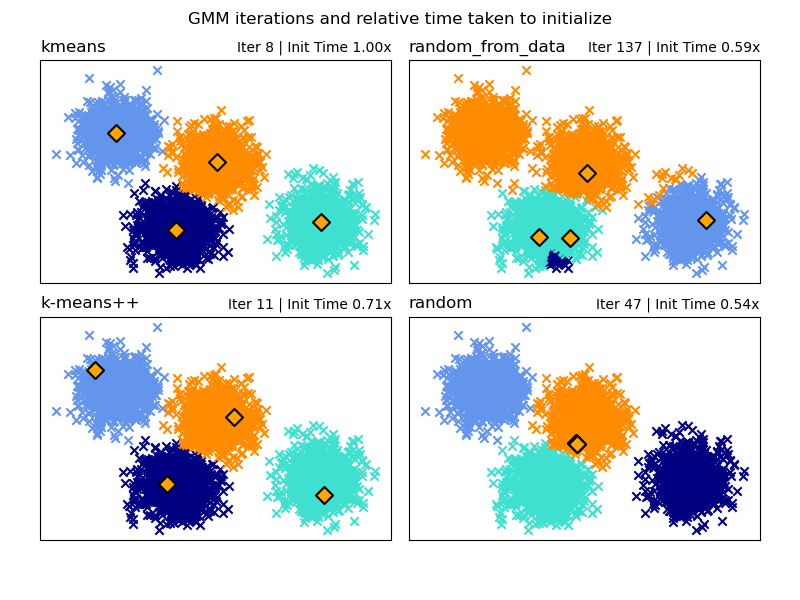
\includegraphics[width=0.9\textwidth]{F4.png}
            \caption{GMM算法在不同初始化策略下的迭代次数与收敛情况对比,其中k-means++是常用的高效初始化方法。}
            \label{fig:gmm_initialization_comparison}
        \end{figure}
        
        \item \textbf{应用:异常检测。} GMM学习了正常数据的分布后,可用于异常检测。对于一个新的数据点,如果其在所有高斯成分下的概率密度(即似然度)都非常低,那么它就很可能是一个异常点(如图 \ref{fig:gmm_log_likelihood})。这在识别欺诈交易或洗钱行为中非常有效。

        \begin{figure}[htbp]
            \centering
            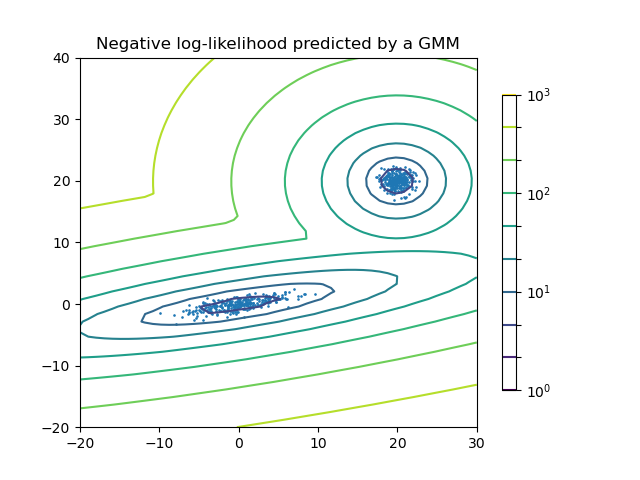
\includegraphics[width=0.7\textwidth]{F3.png}
            \caption{由GMM预测的负对数似然度等高线图。离中心区域越远的数据点,其似然度越低,越可能是异常点。}
            \label{fig:gmm_log_likelihood}
        \end{figure}

        \item \textbf{进阶应用:贝叶斯GMM。} 传统GMM需要预先指定聚类的数量$K$。而\textbf{贝叶斯高斯混合模型(Bayesian GMM)}利用\textbf{狄利克雷过程(Dirichlet Process)}作为先验,可以从数据中自动推断出最合适的聚类数量。如图 \ref{fig:bayesian_gmm_comparison} 所示,不同的先验假设($\gamma_0$)会引导模型发现不同数量的簇,这赋予了模型更大的灵活性。图 \ref{fig:gmm_vs_bayesian_gmm} 和图 \ref{fig:gmm_dirichlet_process_detailed} 提供了标准GMM与贝叶斯GMM在聚类效果上的直观对比。

    \end{itemize}

    \begin{figure}[htbp]
        \centering
        \begin{subfigure}[b]{\textwidth}
            \centering
            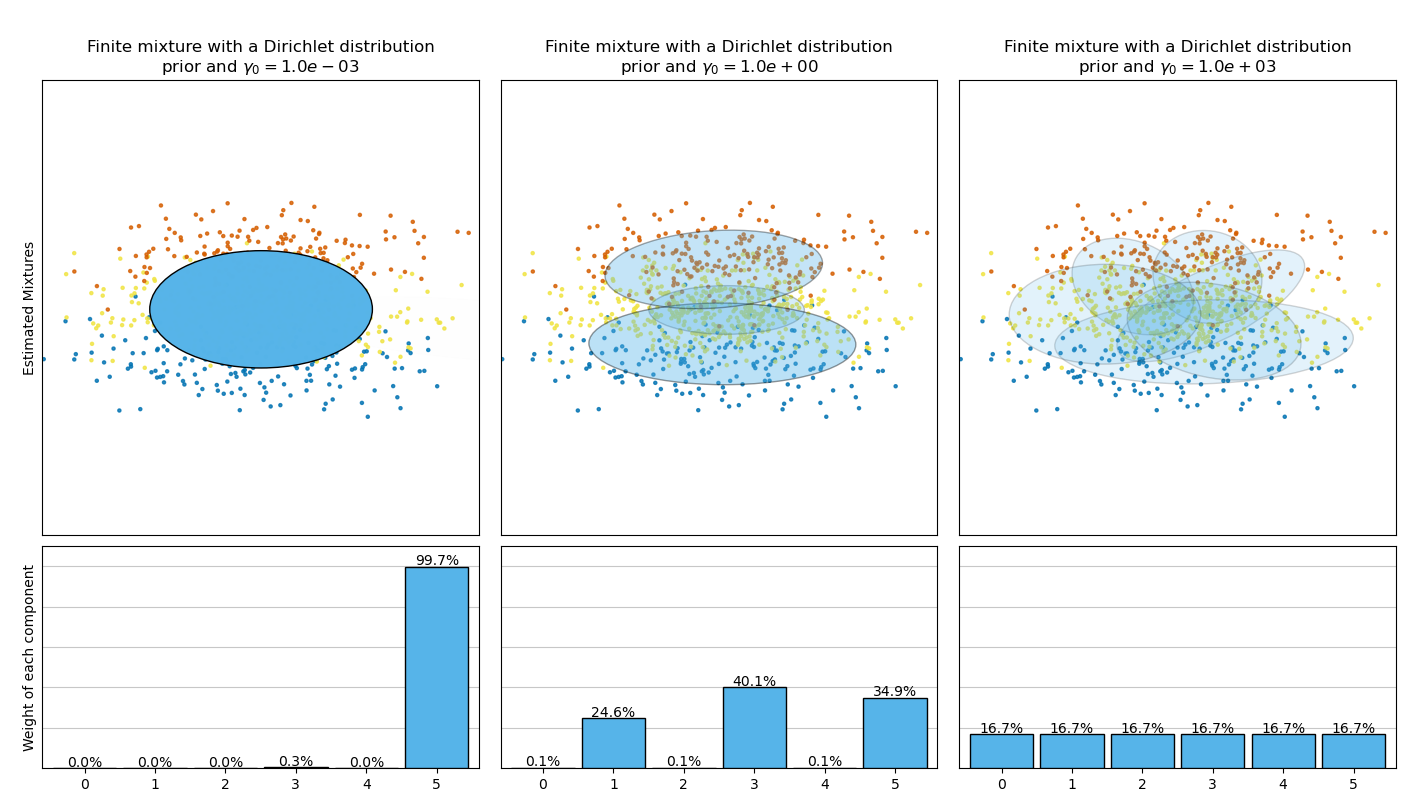
\includegraphics[width=\textwidth]{F1.png}
            \caption{有限混合模型,展示了先验强度$\gamma_0$较小时,模型倾向于发现更少的簇。}
            \label{fig:finite_mixture_dirichlet}
        \end{subfigure}
        \vfill
        \begin{subfigure}[b]{\textwidth}
            \centering
            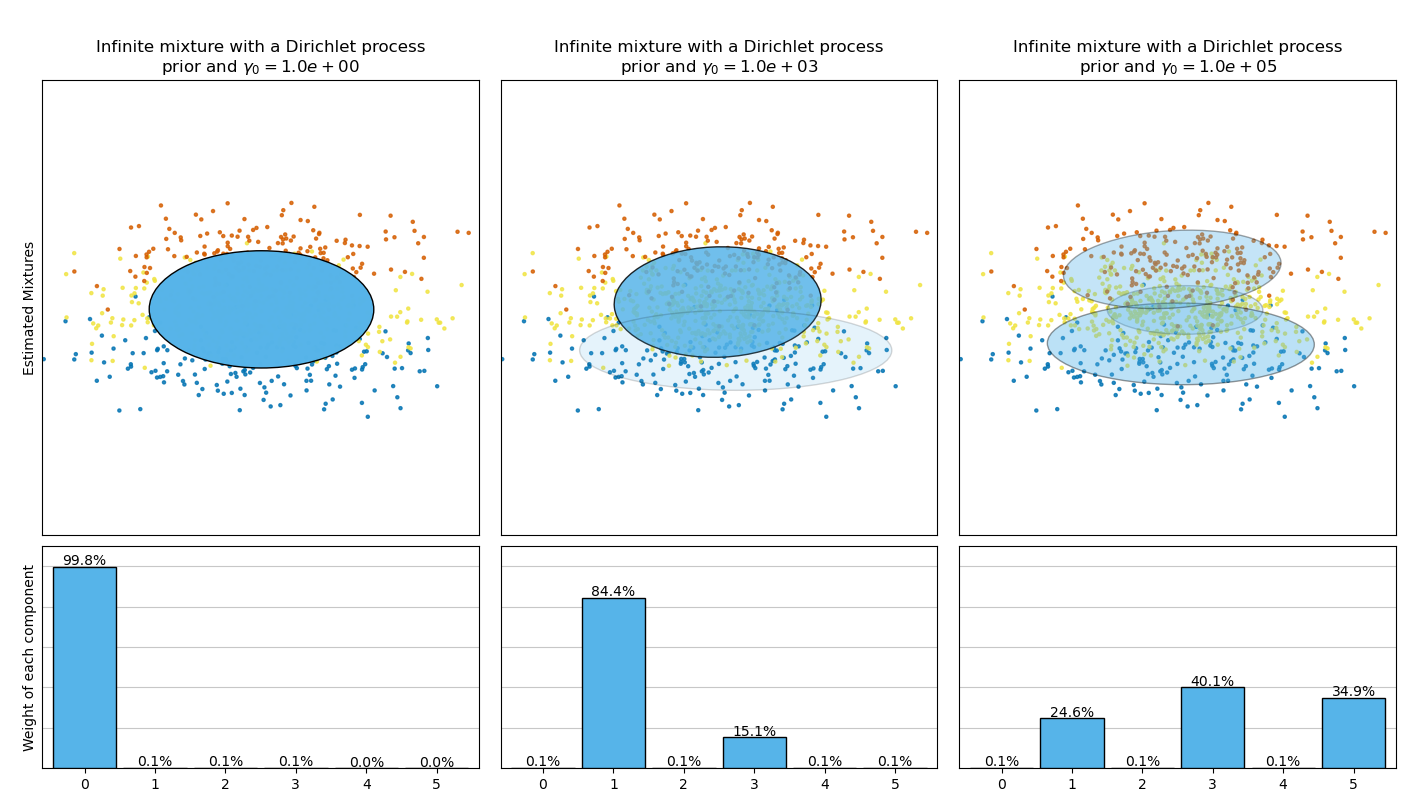
\includegraphics[width=\textwidth]{F2.png}
            \caption{无限混合模型,展示了随着先验强度$\gamma_0$增大,模型能够发现更多、更细粒度的簇。}
            \label{fig:infinite_mixture_dirichlet}
        \end{subfigure}
        \caption{贝叶斯GMM中狄利克雷过程先验对聚类数量的影响对比。}
        \label{fig:bayesian_gmm_comparison}
    \end{figure}

    \begin{figure}[htbp]
        \centering
        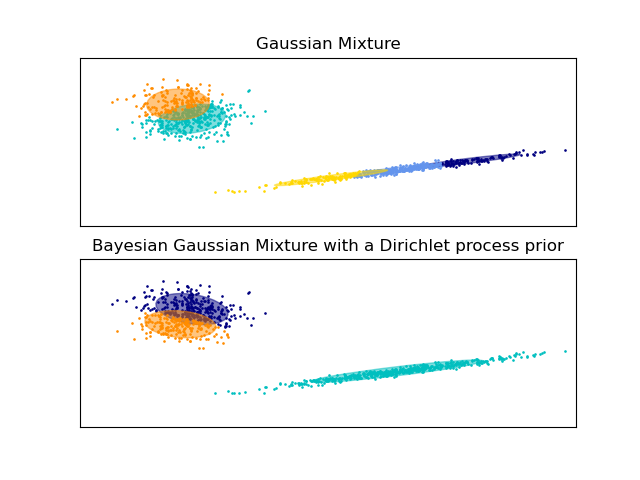
\includegraphics[width=0.8\textwidth]{F6.png}
        \caption{标准GMM(上)与使用狄利克雷过程先验的贝叶斯GMM(下)的聚类结果对比。}
        \label{fig:gmm_vs_bayesian_gmm}
    \end{figure}
    
    \begin{figure}[htbp]
        \centering
        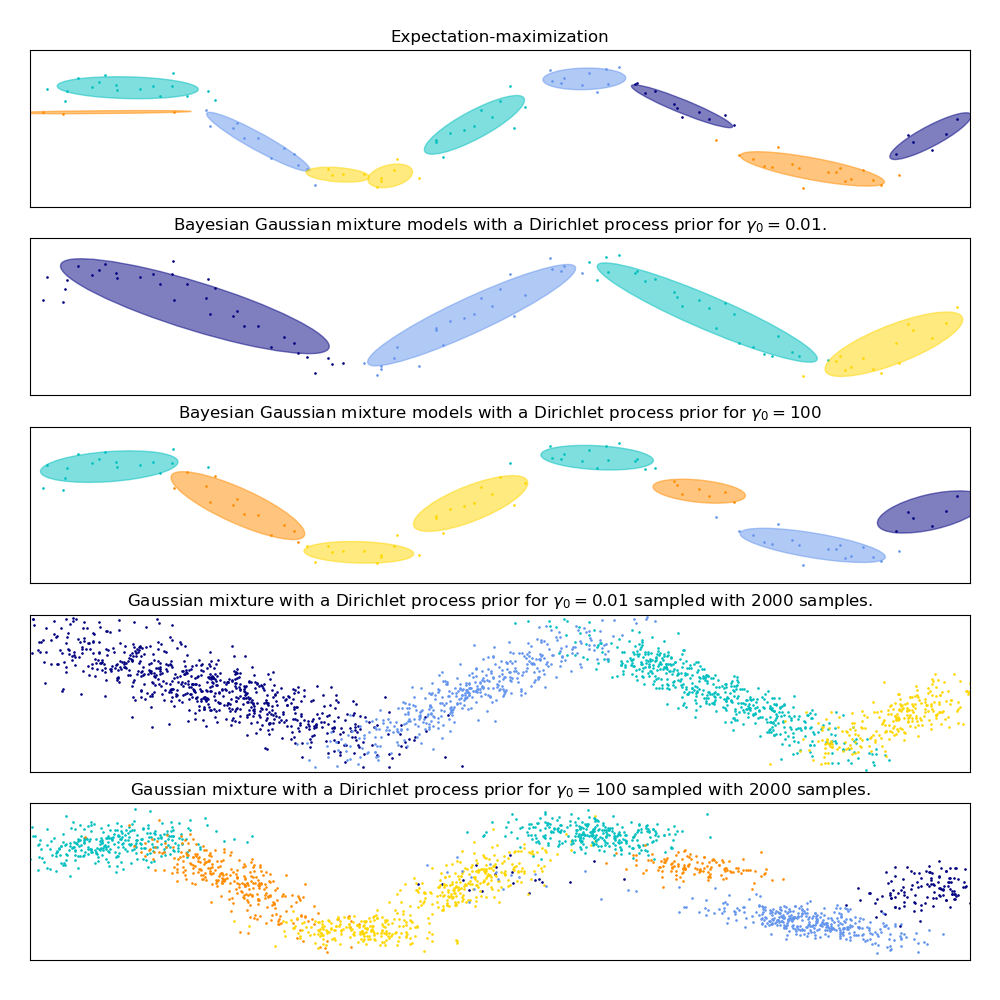
\includegraphics[width=0.9\textwidth]{F8.png}
        \caption{EM算法与不同先验强度下的贝叶斯GMM的详细聚类效果对比。}
        \label{fig:gmm_dirichlet_process_detailed}
    \end{figure}
    
    \subsubsection{量化交易与算法交易}
    人工智能在量化交易领域的应用,旨在通过算法自动执行高频、复杂的交易策略,以捕捉市场中稍纵即逝的套利机会。
    \begin{itemize}
        \item \textbf{核心技术:} \textbf{强化学习(Reinforcement Learning, RL)}是该领域的前沿技术。AI智能体(Agent)被训练在一个模拟的市场环境中,其目标是学习一个最优的交易策略(Policy)$\pi$,以最大化长期的累积收益。此外,用于时间序列预测的\textbf{LSTM}和\textbf{Transformer}模型也被广泛用于预测资产价格的短期波动。

        \item \textbf{原理与公式:} 在强化学习框架下,智能体的目标是找到一个策略 $\pi(a_t | s_t)$,即在给定的市场状态 $s_t$(包含当前价格、交易量、新闻情感等信息)下,采取能带来最大化未来预期回报的行动 $a_t$(买入、卖出或持有)。其优化的目标函数(价值函数)可以表示为:
        $$
        V^\pi(s_t) = \mathbb{E}_\pi \left[ \sum_{k=0}^{\infty} \gamma^k R_{t+k+1} | S_t=s_t \right]
        $$
        其中,$R_{t+k+1}$ 是在未来第 $k$ 步执行策略后获得的奖励(即投资回报),$\gamma$ 是一个折扣因子,用于平衡即时奖励与远期奖励的重要性。AI通过不断的模拟交易和策略迭代(如Q-learning或Policy Gradient等算法),最终学会在复杂的市场动态中做出最优决策。
    \end{itemize}
    
    \subsubsection{智能投顾与财富管理}
    智能投顾(Robo-Advisor)是人工智能与金融服务结合的典范,它利用算法为用户提供自动化的投资组合建议和管理服务,降低了传统财富管理的门槛。
    \begin{itemize}
        \item \textbf{核心技术:}
            \begin{itemize}
                \item \textbf{用户画像构建:} AI通过分析用户填写的问卷(包含财务状况、投资目标、风险偏好等),结合其消费和行为数据,构建精准的用户画像。
                \item \textbf{资产配置模型:} 这是智能投顾的核心。系统主要应用\textbf{现代投资组合理论(Modern Portfolio Theory, MPT)},通过\textbf{二次规划(Quadratic Programming)}等优化算法,寻找在给定预期收益水平下,风险(即投资组合的方差)最小的资产组合。
                \item \textbf{动态再平衡:} AI系统持续监控市场波动导致的资产偏离,当偏离度超过设定阈值时,自动执行交易,使投资组合重新回到目标配置上。
            \end{itemize}
        \item \textbf{原理与公式:} MPT的核心是构建“有效前沿”(Efficient Frontier)。对于一个包含 $n$ 种资产的投资组合,其预期收益率 $E(R_p)$ 和风险(方差)$\sigma_p^2$ 分别为:
        $$ E(R_p) = \sum_{i=1}^{n} w_i E(R_i) $$
        $$ \sigma_p^2 = \sum_{i=1}^{n} \sum_{j=1}^{n} w_i w_j \text{Cov}(R_i, R_j) $$
        其中,$w_i$ 是第 $i$ 种资产的投资权重,$E(R_i)$ 是其预期收益率,$\text{Cov}(R_i, R_j)$ 是资产 $i$ 和 $j$ 收益率的协方差。智能投顾的目标是在满足 $\sum w_i = 1$ 的约束下,通过调整权重 $w_i$ 来求解最优的资产配置方案。
    \end{itemize}
    
    \item \textbf{交通:} 自动驾驶技术是AI在交通领域的核心体现,它通过复杂的感知、决策和控制系统,致力于提升道路安全与运输效率。其技术核心在于\textbf{多传感器融合},以确保系统对周围环境有全面、准确的理解。
    
    \subsubsection{自动驾驶中的多传感器融合与感知}
    自动驾驶的“眼睛”和“耳朵”由多种传感器构成,单一传感器存在局限性(如摄像头受光照影响,雷达分辨率低),因此必须将它们的信息融合起来,形成一个比任何单一来源都更可靠的环境表征。
    \begin{itemize}
        \item \textbf{核心技术概览:} 深度学习算法是传感器融合与感知的基石。如图 \ref{fig:deep_learning_sensor_fusion_algorithms} 所示,这些算法主要分为两大类:用于处理图像等空间数据的\textbf{卷积神经网络(CNN)},以及用于处理序列数据的\textbf{循环神经网络(RNN)}。
        
        \begin{figure}[htbp]
            \centering
            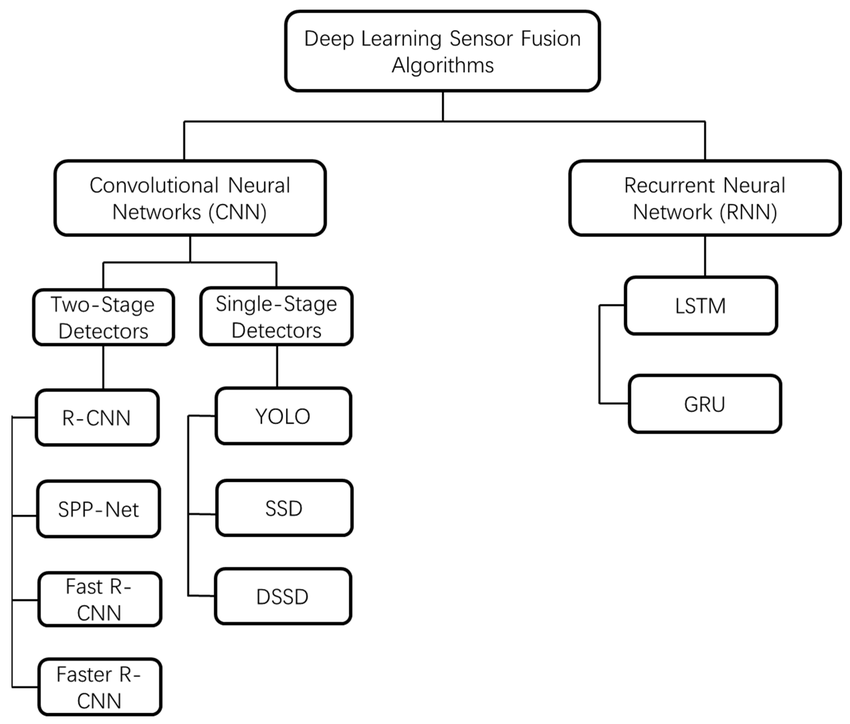
\includegraphics[width=0.8\textwidth]{DR6.png}
            \caption{用于传感器融合的深度学习算法分类,展示了CNN和RNN两大技术分支及其典型模型。}
            \label{fig:deep_learning_sensor_fusion_algorithms}
        \end{figure}
        
        \item \textbf{端到端融合架构:} 现代自动驾驶系统倾向于采用端到端的学习模型。如图 \ref{fig:multisensor_fusion_architecture} 所示,系统并行处理来自不同传感器的数据流:
        \begin{itemize}
            \item \textbf{RGB图像} 由视觉模型(如\textbf{ViT},视觉Transformer)处理。
            \item \textbf{深度图像} 由\textbf{DenseNet}等CNN模型处理。
            \item \textbf{激光雷达点云} 由专门的\textbf{PointNet}系列模型处理。
        \end{itemize}
        这些模型各自提取特征,然后通过一个融合模块(如图中的SCP和RTA)将特征进行整合,最终输出驾驶决策(如方向、油门、刹车)。

        \begin{figure}[htbp]
            \centering
            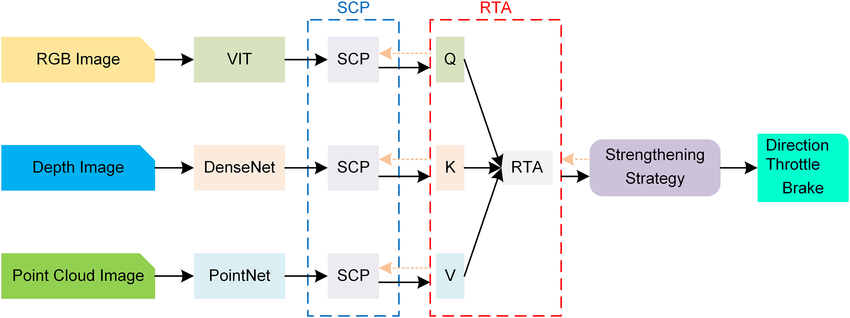
\includegraphics[width=0.95\textwidth]{DR1.png}
            \caption{一个典型的自动驾驶多传感器融合架构,展示了从RGB图像、深度图像和点云输入,经过并行处理与融合,到最终输出驾驶策略的完整流程。}
            \label{fig:multisensor_fusion_architecture}
        \end{figure}
        
        \item \textbf{感知模块详解:}
        \begin{itemize}
            \item \textbf{图像处理:} CNN通过卷积操作提取图像特征。一个基本的卷积运算可以表示为:
            $$
            (f * g)(i,j) = \sum_m \sum_n f(m,n) g(i-m, j-n)
            $$
            其中 $f$ 是输入图像,$g$ 是卷积核。通过堆叠多个卷积层和池化层,模型能学习到从边缘到物体的层次化特征,如图 \ref{fig:cnn_for_depth_image} 所示。更先进的模型如\textbf{视觉Transformer (ViT)}(架构如图 \ref{fig:vision_transformer_architecture})则通过自注意力机制捕捉图像的全局依赖关系。

            \begin{figure}[htbp]
            \centering
            \begin{subfigure}[b]{0.48\textwidth}
                \centering
                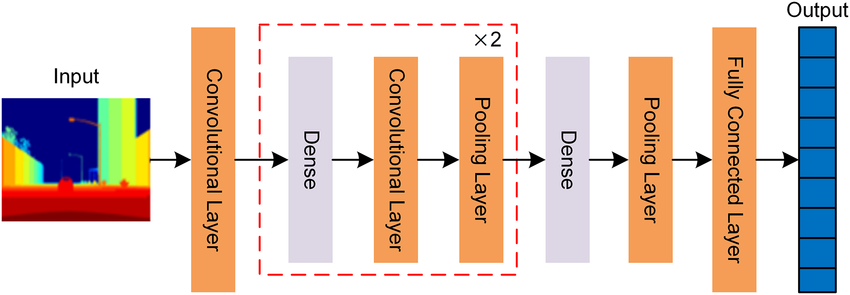
\includegraphics[width=\textwidth]{DR3.png}
                \caption{一个用于处理深度图像的CNN架构示例。}
                \label{fig:cnn_for_depth_image}
            \end{subfigure}
            \hfill
            \begin{subfigure}[b]{0.48\textwidth}
                \centering
                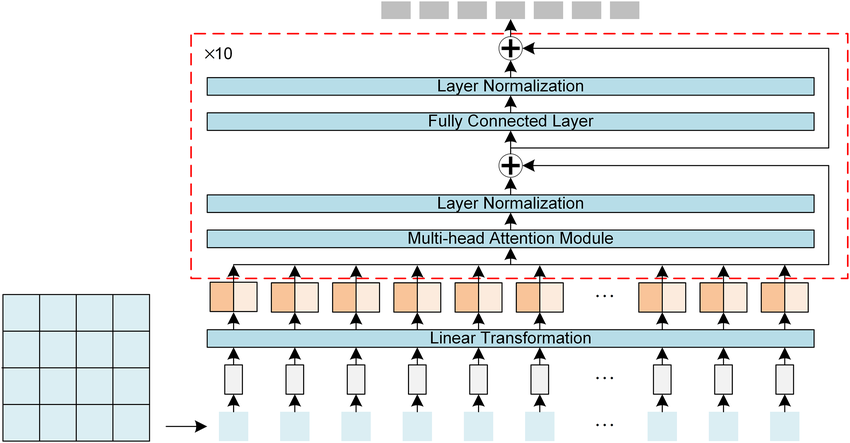
\includegraphics[width=\textwidth]{DR2.png}
                \caption{视觉Transformer中的一个核心Encoder模块。}
                \label{fig:vision_transformer_architecture}
            \end{subfigure}
            \caption{用于图像处理的两种主流深度学习模型架构。}
            \label{fig:image_processing_architectures}
            \end{figure}

            \item \textbf{点云处理:} 对于LiDAR产生的3D点云,\textbf{PointNet}(架构如图 \ref{fig:pointnet_architecture})等模型通过直接处理点集,学习其空间分布特征,有效解决了点云数据无序性和不规则性的问题。
            
            \begin{figure}[htbp]
                \centering
                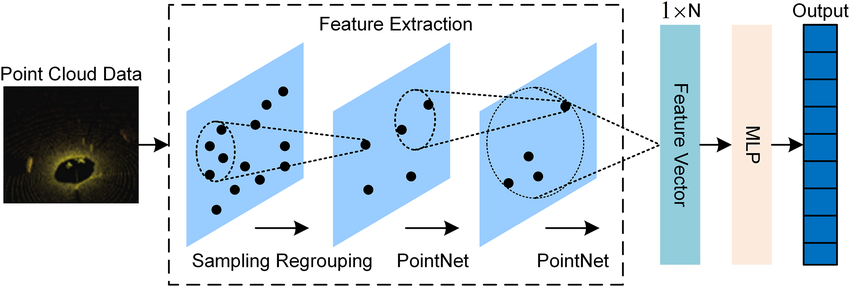
\includegraphics[width=0.9\textwidth]{DR4.png}
                \caption{PointNet模型处理激光雷达点云数据的流程示意图。}
                \label{fig:pointnet_architecture}
            \end{figure}
            
            \item \textbf{特征融合机制:} 来自不同传感器的特征流需要有效融合。这通常通过拼接(Concatenation)、逐元素相加或更复杂的\textbf{注意力机制}(Attention Mechanism)来实现。图 \ref{fig:feature_fusion_mechanism} 展示了一种可能的特征融合过程。

             \begin{figure}[htbp]
                \centering
                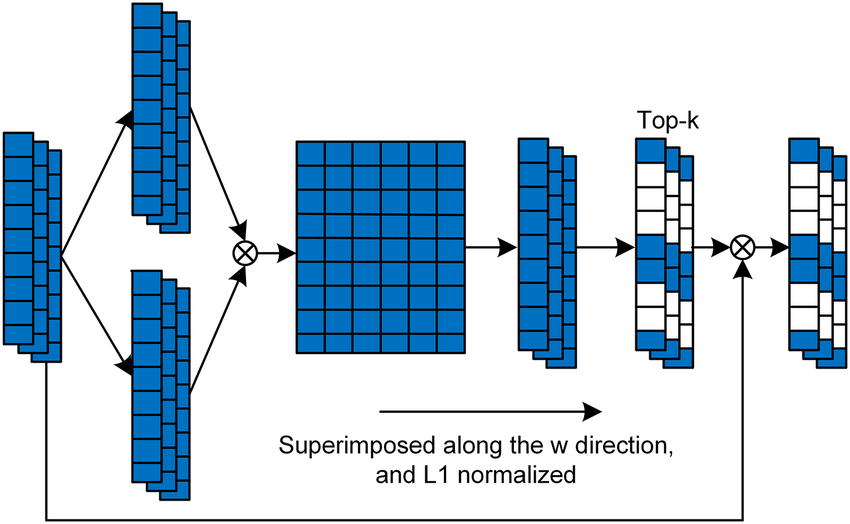
\includegraphics[width=0.8\textwidth]{DR5.png}
                \caption{一种特征融合机制的示意图,可能代表了注意力或特征叠加操作。}
                \label{fig:feature_fusion_mechanism}
            \end{figure}
            
        \end{itemize}
    \end{itemize}

    \subsubsection{定位与导航:车辆的自我感知}
    除了感知外部环境,车辆还必须精确知道自身的位置和姿态。这同样依赖于多传感器融合,但更侧重于惯性导航系统(INS)、全球导航卫星系统(GNSS)和里程计等。
    \begin{itemize}
        \item \textbf{核心技术:卡尔曼滤波(Kalman Filter)}及其变体(如扩展卡尔曼滤波EKF、无迹卡尔曼滤波UKF)是该领域的核心算法。它是一种最优递归数据处理算法,能在一系列不完全和包含噪声的测量中,估计动态系统的状态。
        \item \textbf{原理与架构:} 系统通过一个主滤波器融合来自不同子系统(如SINS、里程计OD、激光多普勒测速仪LDV)的信息,如图 \ref{fig:kalman_filter_fusion_framework} 所示。其核心的状态更新方程为:
        $$
        \hat{x}_k = \hat{x}_{k|k-1} + K_k (z_k - H_k \hat{x}_{k|k-1})
        $$
        其中,$\hat{x}_k$ 是当前时刻的状态估计值,$\hat{x}_{k|k-1}$ 是基于上一时刻状态的预测值,$z_k$ 是当前时刻的测量值,$K_k$ 是卡尔曼增益,它平衡了预测值和测量值的不确定性。图 \ref{fig:inertial_system_alignment_flowchart} 展示了一个利用卡尔曼精对准的惯性系统校准流程,而图 \ref{fig:sensor_calibration_topologies} 则显示了进行有效融合前,必须完成的多传感器标定步骤。
    \end{itemize}

    \begin{figure}[htbp]
        \centering
        \begin{subfigure}[b]{0.48\textwidth}
            \centering
            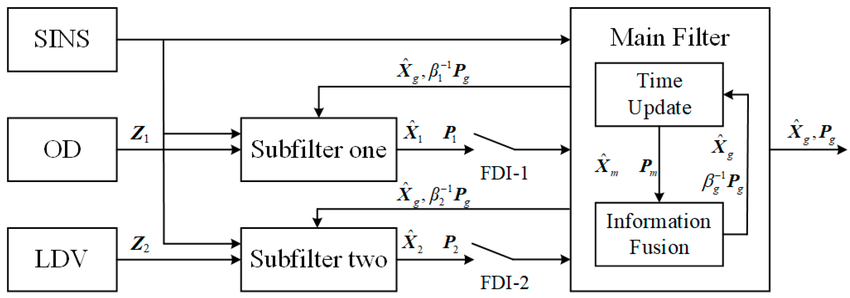
\includegraphics[width=\textwidth]{DR7.png}
            \caption{基于卡尔曼滤波的多传感器融合框架。}
            \label{fig:kalman_filter_fusion_framework}
        \end{subfigure}
        \hfill
        \begin{subfigure}[b]{0.48\textwidth}
            \centering
            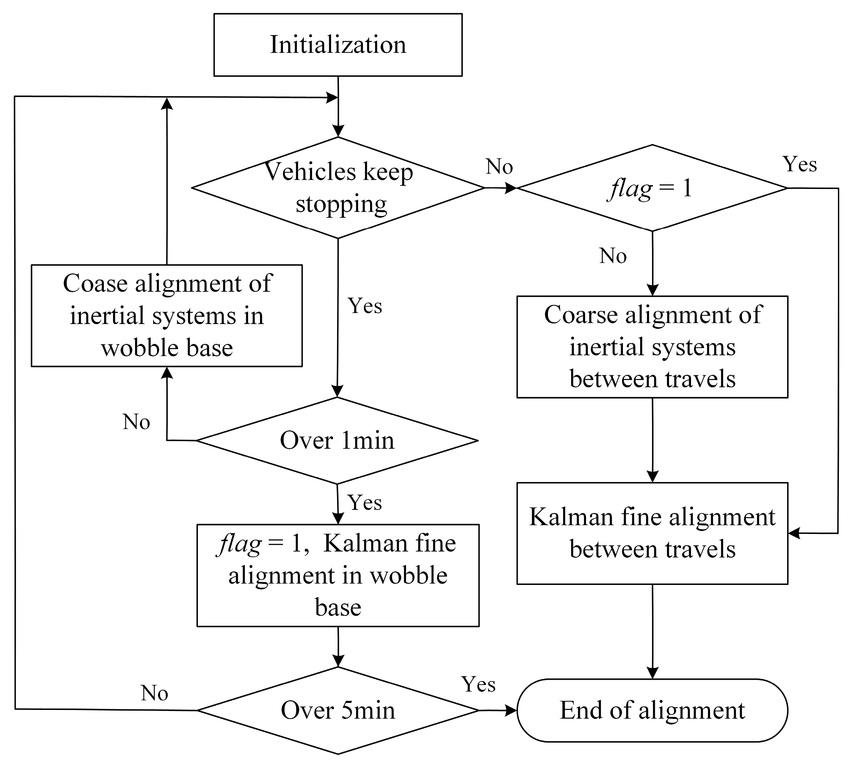
\includegraphics[width=\textwidth]{DR9.png}
            \caption{惯性系统(如SINS)的对准流程图。}
            \label{fig:inertial_system_alignment_flowchart}
        \end{subfigure}
        \caption{车辆定位中的传感器信息融合与校准流程。}
        \label{fig:localization_fusion_calibration}
    \end{figure}
    
    \begin{figure}[htbp]
        \centering
        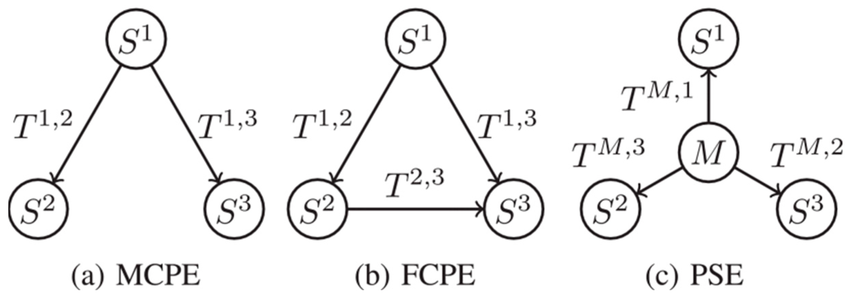
\includegraphics[width=0.7\textwidth]{DR8.png}
        \caption{自动驾驶系统中常见的多传感器标定拓扑结构。}
        \label{fig:sensor_calibration_topologies}
    \end{figure}
    
    \item \textbf{工业:} 在工业4.0的浪潮中,人工智能正驱动着制造业向智能化、柔性化和高效化转型,其核心应用体现在智能制造和预测性维护两大方面。

    \subsubsection{智能制造与自动化}
    AI技术通过赋予机器“视觉”和“决策能力”,实现了生产线的高度自动化和智能化。
    \begin{itemize}
        \item \textbf{核心技术:}
            \begin{itemize}
                \item \textbf{AI质检(视觉检测):} 利用高分辨率相机和\textbf{卷积神经网络(CNN)},AI可以替代人眼完成产品表面缺陷的检测。模型如YOLO(You Only Look Once)或Faster R-CNN能够实时地在生产线上定位并识别出划痕、污点、裂纹等微小瑕疵,准确率和速度远超人工。
                \item \textbf{机器人协同作业:} 工业机器人通过\textbf{强化学习}学会复杂的操作任务,如精密装配和焊接。通过在模拟环境中进行大量“试错”训练,机器人能够学习到最优的动作序列,以适应不同工件和生产需求。
                \item \textbf{生产流程优化:} AI分析整个生产流程的数据,识别瓶颈工序,并通过\textbf{运筹学优化算法}(如模拟退火、遗传算法)对生产计划、物料调度进行优化,以达到生产效率的最大化。
            \end{itemize}
    \end{itemize}

    \subsubsection{预测性维护(Predictive Maintenance, PdM)}
    预测性维护旨在设备发生故障前,通过AI分析其运行数据,提前预测故障并安排维修,从而最大限度地减少非计划停机时间,降低维护成本。
    \begin{itemize}
        \item \textbf{核心技术:} 主要基于对设备传感器(如振动、温度、压力传感器)产生的\textbf{时间序列数据}进行分析。
            \begin{itemize}
                \item \textbf{故障预测:} \textbf{长短期记忆网络(LSTM)}或\textbf{门控循环单元(GRU)}等RNN模型非常适合处理这类时间序列数据,它们能够学习设备正常运行时的模式,并预测未来的状态。当预测值与正常阈值出现显著偏差时,系统就会发出预警。
                \item \textbf{剩余使用寿命(RUL)预测:} AI模型可以直接对设备的剩余使用寿命进行回归预测。这是一个典型的回归问题,其目标是学习一个从传感器读数序列到剩余寿命时间的映射函数。
            \end{itemize}
        \item \textbf{原理与公式:} 一个简化的时间序列预测模型可以表示为:
        $$
        \hat{X}_{t+1} = f(X_t, X_{t-1}, \dots, X_{t-k}; \theta)
        $$
        其中,$\hat{X}_{t+1}$ 是对下一时刻传感器读数的预测值,$X_t, \dots, X_{t-k}$ 是过去 $k$ 个时刻的观测值序列,$f$ 是由AI模型(如LSTM)所代表的复杂非线性函数,$\theta$ 是模型参数。通过最小化预测值与真实值之间的误差(如均方误差),模型能够学习到设备状态的演变规律。
    \end{itemize}

    \item \textbf{教育:} 人工智能正逐步渗透到教育的各个环节,通过技术手段推动因材施教和个性化发展,致力于提升学习效率和教育公平。

    \subsubsection{个性化学习与智能推荐}
    AI能够打破“一刀切”的传统教学模式,为每个学生量身定制独特的学习内容和路径。
    \begin{itemize}
        \item \textbf{核心技术:}
            \begin{itemize}
                \item \textbf{知识图谱(Knowledge Graph):} AI首先将学科知识构建成一个由知识点(节点)和它们之间的依赖关系(边)组成的网络。
                \item \textbf{认知诊断与知识追踪(Cognitive Diagnosis \& Knowledge Tracing):} AI通过分析学生的练习、测验和互动数据,利用\textbf{贝叶斯网络}或\textbf{深度学习模型}(如DKT - Deep Knowledge Tracing),动态追踪每个学生对各个知识点的掌握程度。
                \item \textbf{推荐算法:} 基于学生的知识掌握状态和学习目标,AI采用类似电商推荐的\textbf{协同过滤}或\textbf{基于内容的推荐}算法,为学生推荐最适合他们的学习资源(如视频、习题、阅读材料),以弥补薄弱环节或进行拓展学习。
            \end{itemize}
        \item \textbf{原理与概念:} 一个学生 $u$ 对一个知识点 $i$ 的掌握概率 $P(K_i | u)$ 可以通过模型进行估计。推荐系统的目标是找到一个项目 $j$(学习资源),使得该项目能最大化学生的预期知识增益 $E[\Delta K | u, j]$。一个简化的推荐逻辑可以是:
        $$
        \text{Item}^* = \arg\max_{j \in I} \left( w_1 \cdot \text{relevance}(j, u) - w_2 \cdot \text{difficulty}(j, u) \right)
        $$
        其中,$\text{relevance}$衡量资源与学生知识薄弱点的相关性,$\text{difficulty}$衡量资源的难度是否与学生当前水平匹配,$w_1, w_2$为权重。
    \end{itemize}

    \subsubsection{智能辅导系统与自动评估}
    AI充当着24/7在线的智能导师,为学生提供即时帮助,并解放教师的重复性批改工作。
    \begin{itemize}
        \item \textbf{核心技术:}
            \begin{itemize}
                \item \textbf{智能问答(QA):} 基于\textbf{自然语言处理(NLP)}和\textbf{大型语言模型(LLM)},智能辅导系统能够理解学生用自然语言提出的问题,并提供精准的解答或引导性的提示。
                \item \textbf{自动作文评分(Automated Essay Scoring, AES):} AI通过分析大量已评分的作文,学习评分标准。它利用NLP技术提取文本的特征,如词汇丰富度、句子结构复杂度、逻辑连贯性(如使用\textbf{词嵌入}和\textbf{Transformer}模型进行语义分析),然后通过一个\textbf{回归模型}预测作文的分数。
                \item \textbf{口语测评:} AI通过\textbf{语音识别(ASR)}技术将学生的朗读转换为文本,然后从流利度、发音准确性和韵律等多个维度进行综合评分。
            \end{itemize}
    \end{itemize}
\end{itemize}

\subsection{社会生活}
AI技术也深刻改变了人们的日常生活:
\begin{itemize}
    \item \textbf{智能家居:} 智能音箱、智能照明等设备通过AI实现互联互通和智能控制,提升了居住舒适度。
    \item \textbf{个性化推荐:} 电商平台、流媒体服务等利用AI算法分析用户偏好,精准推荐商品、影视内容或音乐,极大丰富了用户的选择。
    \item \textbf{智能助手:} 手机上的语音助手、智能客服等为用户提供便捷的信息查询、日程管理和任务执行服务。
\end{itemize}

\section{伦理、社会与法律挑战}

随着AI应用的深入,其带来的伦理、社会和法律挑战日益凸显,需要全球共同应对。

\subsection{数据隐私与安全}
大数据是AI模型训练的基石,但大规模数据的收集和使用也带来了严峻的隐私泄露风险。如何平衡数据利用与个人隐私保护,是当前亟待解决的问题。

\subsection{算法偏见与公平性}
AI模型的训练数据往往反映了现实世界中的偏见,这可能导致算法在决策过程中产生歧视,例如在招聘、信贷审批等方面出现不公平现象。确保算法的公平性和透明度至关重要。

\subsection{就业市场冲击}
自动化和AI技术的普及将对传统职业构成冲击,部分重复性、程式化的工作可能被机器替代。与此同时,AI的发展也将催生新的职业和就业机会,社会需要适应这一结构性变化。

\subsection{伦理道德与责任}
随着AI系统决策能力的增强,其在医疗、法律等领域的应用将面临复杂的道德困境。当AI系统出现错误或造成损害时,责任应如何归属,是亟待明确的法律和伦理问题。

\subsection{人工智能安全}
AI系统并非完美无缺,其脆弱性可能被恶意利用,例如对抗性攻击可能导致AI模型做出错误判断。此外,AI的潜在滥用风险,如用于自动化武器系统,也引发了广泛担忧。

\section{AI治理与政策}

为应对AI带来的挑战,全球各国正在积极探索和实践AI治理框架和政策。

\subsection{全球各国探索与实践}
\begin{itemize}
    \item \textbf{欧盟:} 欧盟在AI伦理准则和法规制定方面走在前列,例如《人工智能法案》旨在规范AI的高风险应用。
    \item \textbf{美国:} 美国注重通过行业自律和政府指导相结合的方式推动AI发展,并关注AI的国家安全应用。
    \item \textbf{中国:} 中国在AI发展方面展现出强大的国家战略,并积极推动AI伦理规范和标准制定。
\end{itemize}

\subsection{国际合作与全球治理的重要性}
AI技术具有无国界性,其影响是全球性的。因此,国际社会需要加强合作,共同制定AI伦理准则、技术标准和法律框架,以确保AI的健康、可持续发展。

\section{未来趋势与展望}

人工智能的未来发展充满无限可能,也将对人类社会产生深远影响。

\subsection{通用人工智能(AGI)的潜在路径与挑战}
通用人工智能(Artificial General Intelligence, AGI)是AI研究的终极目标之一,它旨在使AI系统具备人类的智能水平,能够完成各种认知任务,甚至在未曾明确编程的领域展现出学习、理解和解决问题的能力。AGI的实现路径和潜在挑战是当前AI领域研究的热点。

目前,AGI的潜在路径主要包括:
\begin{itemize}
    \item \textbf{符号主义与连接主义的融合:} 结合传统符号AI的逻辑推理能力与深度学习的模式识别能力,构建既能进行高层抽象推理,又能从大量数据中学习的混合系统。这可能涉及将知识图谱、逻辑编程等与神经网络相结合。
    \item \textbf{大规模预训练模型:} 延续当前大型语言模型(LLMs)和多模态模型的发展路线,通过海量数据和计算资源训练超大规模模型,期望能通过“涌现能力”达到通用智能。这依赖于模型的规模效应和更高效的训练算法。
    \item \textbf{具身智能与强化学习:} 强调AI系统与物理世界的交互,通过具身(embodied)体验和强化学习(Reinforcement Learning, RL)来学习常识、因果关系和复杂技能,类似于人类儿童通过探索世界来学习。
\end{itemize}

AGI面临的挑战是巨大的:
\begin{itemize}
    \item \textbf{常识推理与因果理解:} 现有AI模型在处理常识性问题和理解因果关系方面仍显不足,这对于通用智能至关重要。
    \item \textbf{学习效率与数据需求:} 现有深度学习模型通常需要海量数据进行训练,而人类往往能从少量样本中快速学习并泛化。
    \item \textbf{可解释性与透明度:} 随着模型复杂性增加,其决策过程变得不透明,难以理解和信任。
    \item \textbf{安全与控制:} 如何确保AGI系统与人类价值观对齐,防止其产生意料之外的行为,是核心的安全挑战。
    \item \textbf{计算资源瓶颈:} 训练和运行AGI可能需要前所未有的计算能力和能源消耗。
\end{itemize}

为了更深入地理解AGI的潜力与挑战,研究者们通过各种实验和模型来评估其在不同学习场景下的表现。以下图表展示了一些关键的发现和概念:

\begin{figure}[H]
    \centering
    \begin{subfigure}[b]{0.49\textwidth}
        \centering
        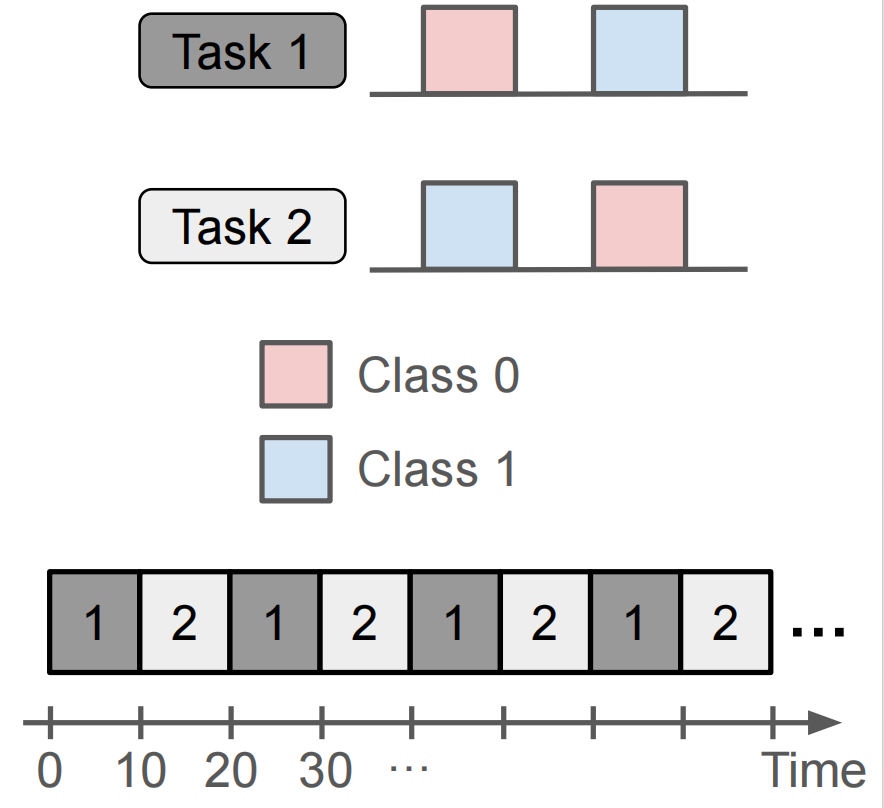
\includegraphics[width=\textwidth]{AGI2.png}
        \caption{周期性与线性任务中数据分布示例}
        \label{fig:agi_task_distribution}
    \end{subfigure}
    \hfill
    \begin{subfigure}[b]{0.49\textwidth}
        \centering
        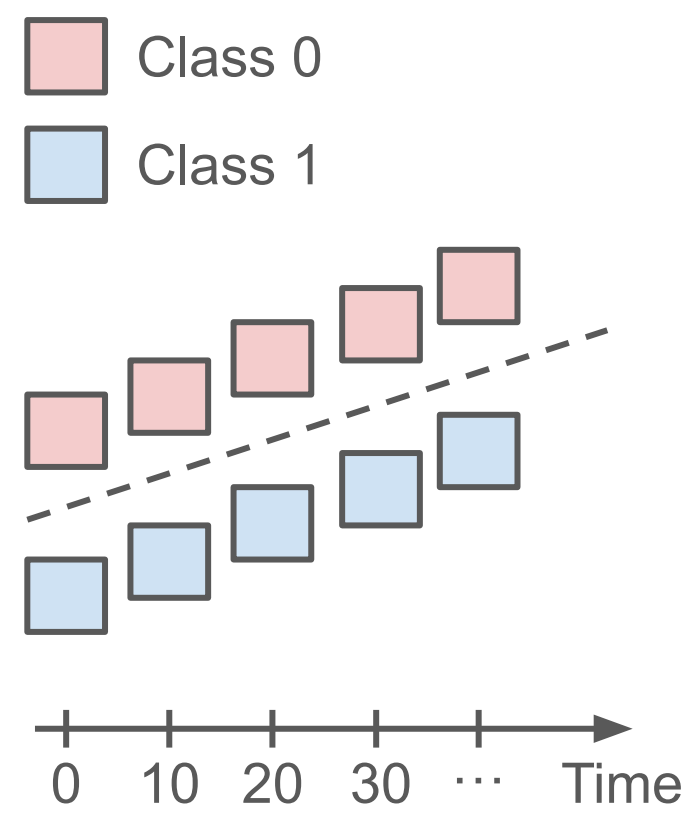
\includegraphics[width=\textwidth]{AGI4.png}
        \caption{随时间变化的类别分布}
        \label{fig:agi_time_varying_classes}
    \end{subfigure}
    \caption{通用人工智能任务中的数据特性与挑战。左图展示了在不同任务(Task 1, Task 2)下,数据点类别(Class 0, Class 1)的周期性与线性变化,反映了AGI需要适应不同时间动态的数据。右图进一步细化了数据点类别随时间的线性演变,这对于模型在动态环境中学习和泛化提出了挑战。}
    \label{fig:agi_data_characteristics}
\end{figure}

\begin{figure}[H]
    \centering
    \begin{subfigure}[b]{0.49\textwidth}
        \centering
        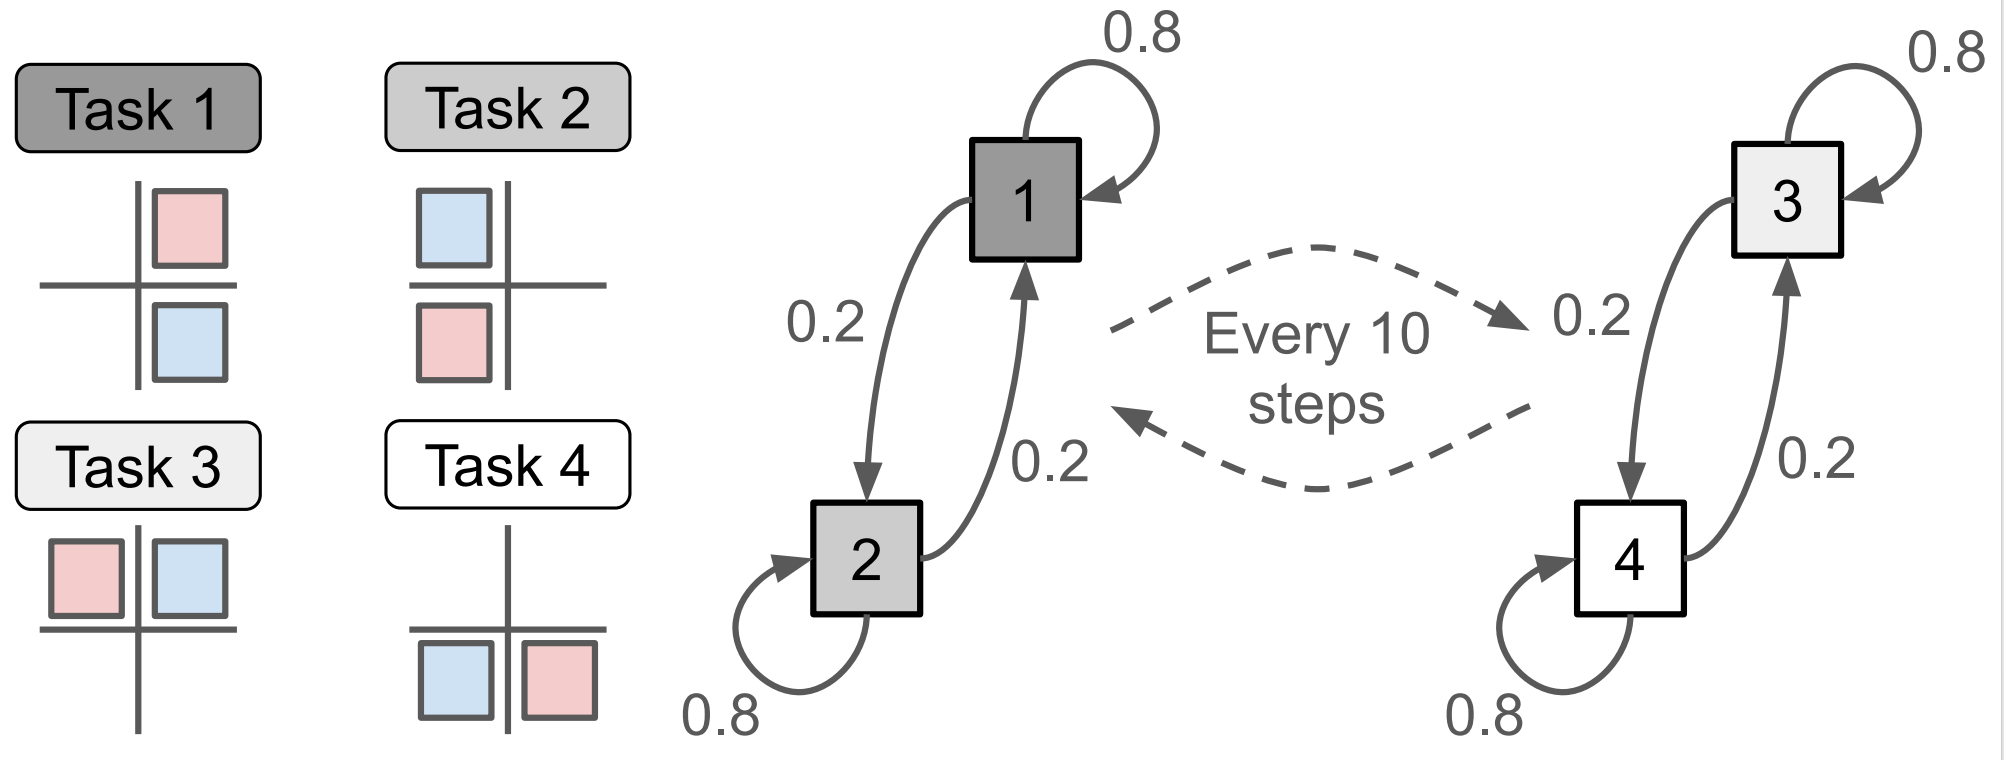
\includegraphics[width=\textwidth]{AGI6.png}
        \caption{多任务与状态转移}
        \label{fig:agi_multi_task_states}
    \end{subfigure}
    \hfill
    \begin{subfigure}[b]{0.49\textwidth}
        \centering
        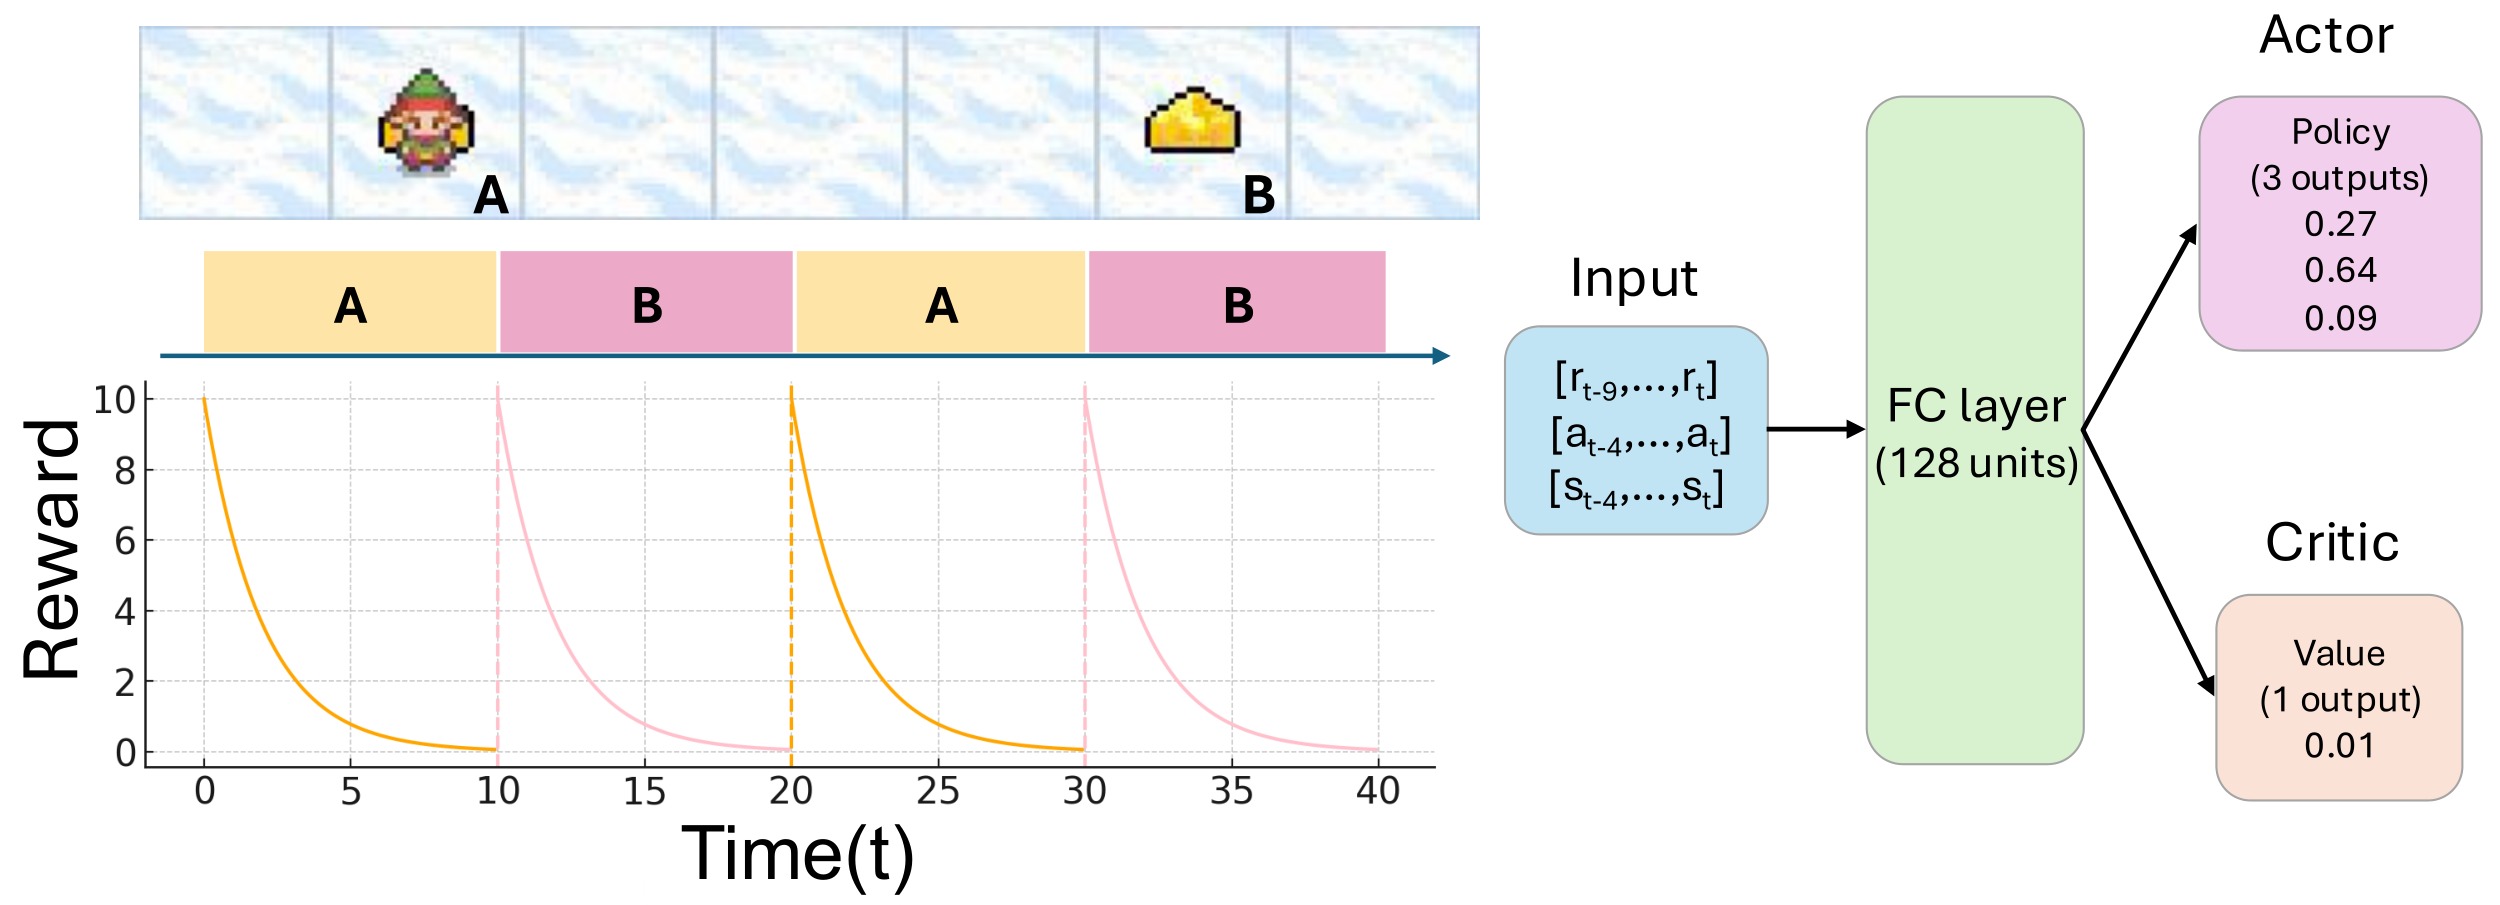
\includegraphics[width=\textwidth]{AGI7.png}
        \caption{强化学习中的Actor-Critic架构与任务奖励}
        \label{fig:agi_actor_critic}
    \end{subfigure}
    \caption{通用智能体学习环境与架构。左图展示了不同任务(Task 1-4)的配置,以及在不同任务状态之间转换的概率,突出了AGI在多任务学习和任务切换方面的能力需求。右图则描绘了强化学习中Actor-Critic模型的输入、网络层和输出,以及智能体在不同任务阶段的奖励变化,是AGI实现复杂行为控制的典型范式。}
    \label{fig:agi_learning_environments_architectures}
\end{figure}

AGI的性能评估不仅关注其在特定任务上的准确率,更关注其在未知或动态环境下的适应性和泛化能力。以下图表展示了模型在风险预测和学习效率方面的表现:

\begin{figure}[H]
    \centering
    \begin{subfigure}[b]{0.49\textwidth}
        \centering
        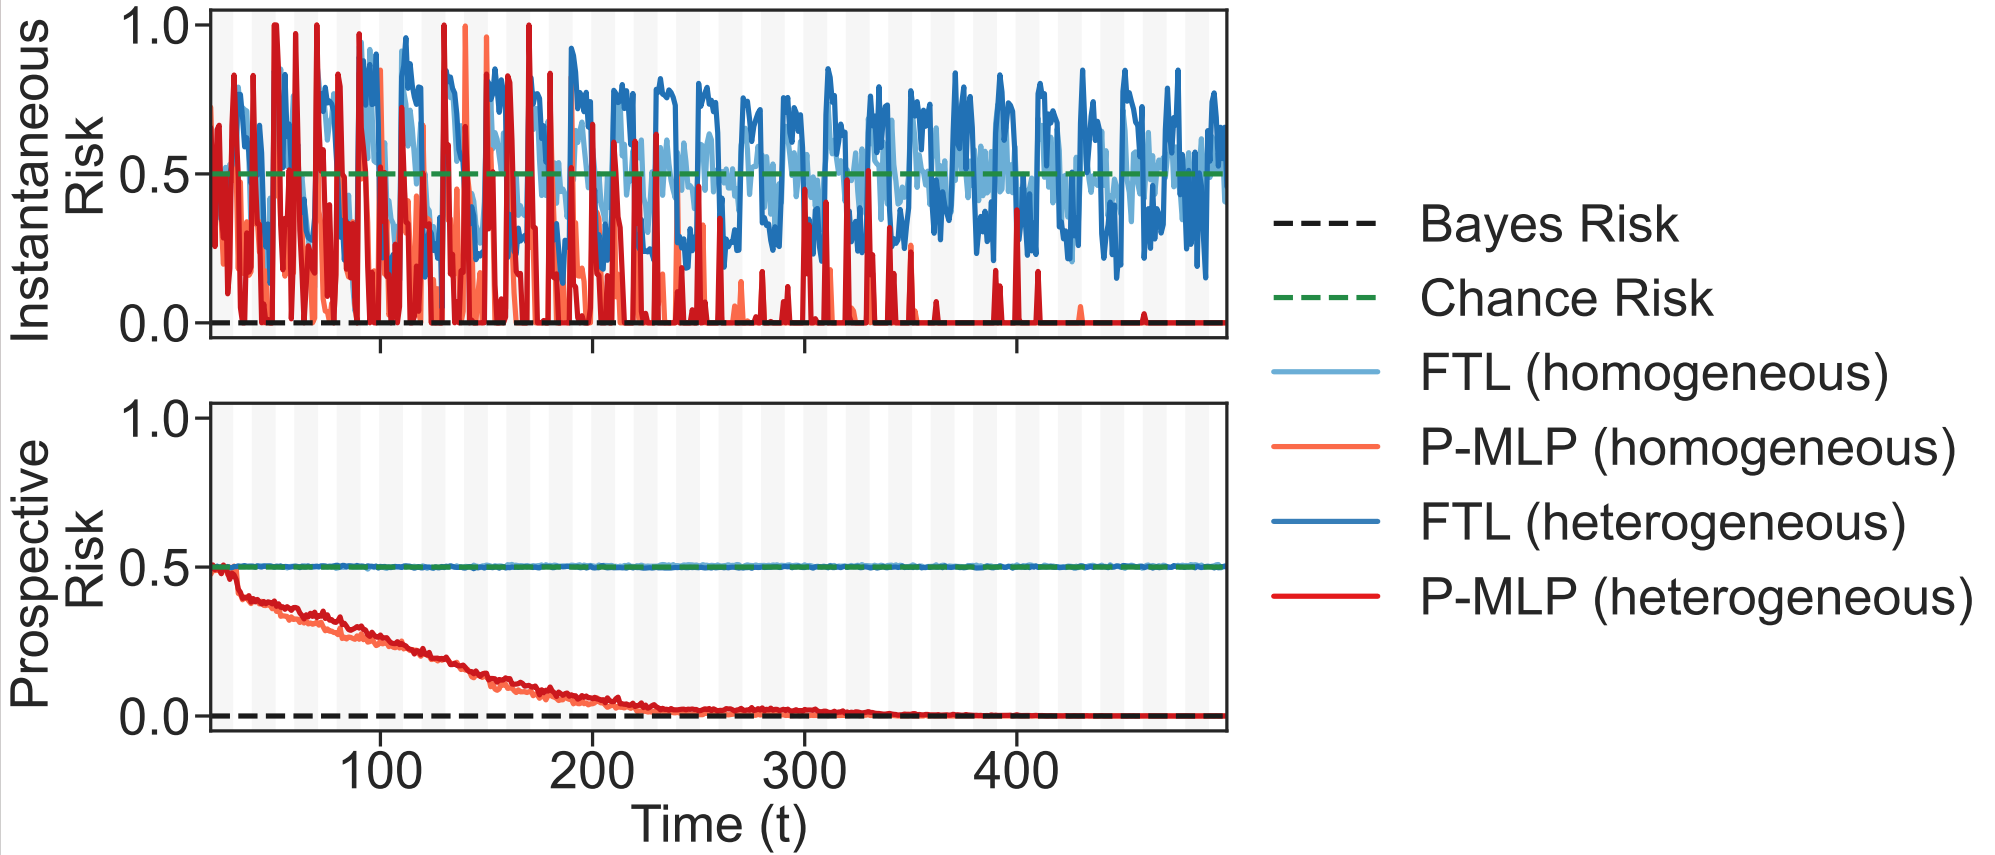
\includegraphics[width=\textwidth]{AGI1.png}
        \caption{异构环境中的即时与预期风险}
        \label{fig:agi_heterogeneous_risk}
    \end{subfigure}
    \hfill
    \begin{subfigure}[b]{0.49\textwidth}
        \centering
        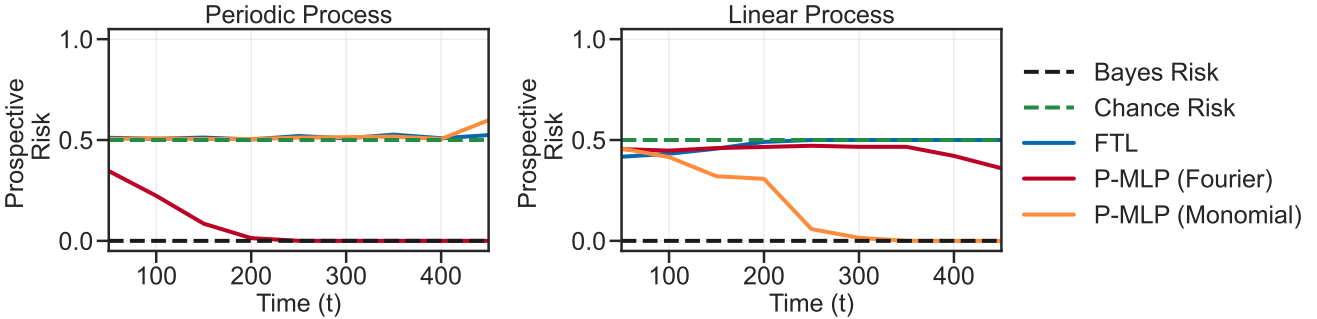
\includegraphics[width=\textwidth]{AGI3.png}
        \caption{周期性与线性过程中的预期风险}
        \label{fig:agi_periodic_linear_risk}
    \end{subfigure}
    \caption{通用智能体在不同数据环境中的风险表现。左图对比了不同算法(FTL, P-MLP)在同构和异构环境下的即时风险和预期风险,展示了模型在处理复杂、非稳定数据时的鲁棒性。右图则细致分析了P-MLP模型在周期性和线性过程中的预期风险,表明其在特定数据模式下能有效降低风险,接近最优水平。}
    \label{fig:agi_risk_performance_comparison}
\end{figure}

\begin{figure}[H]
    \centering
    \begin{subfigure}[b]{0.49\textwidth}
        \centering
        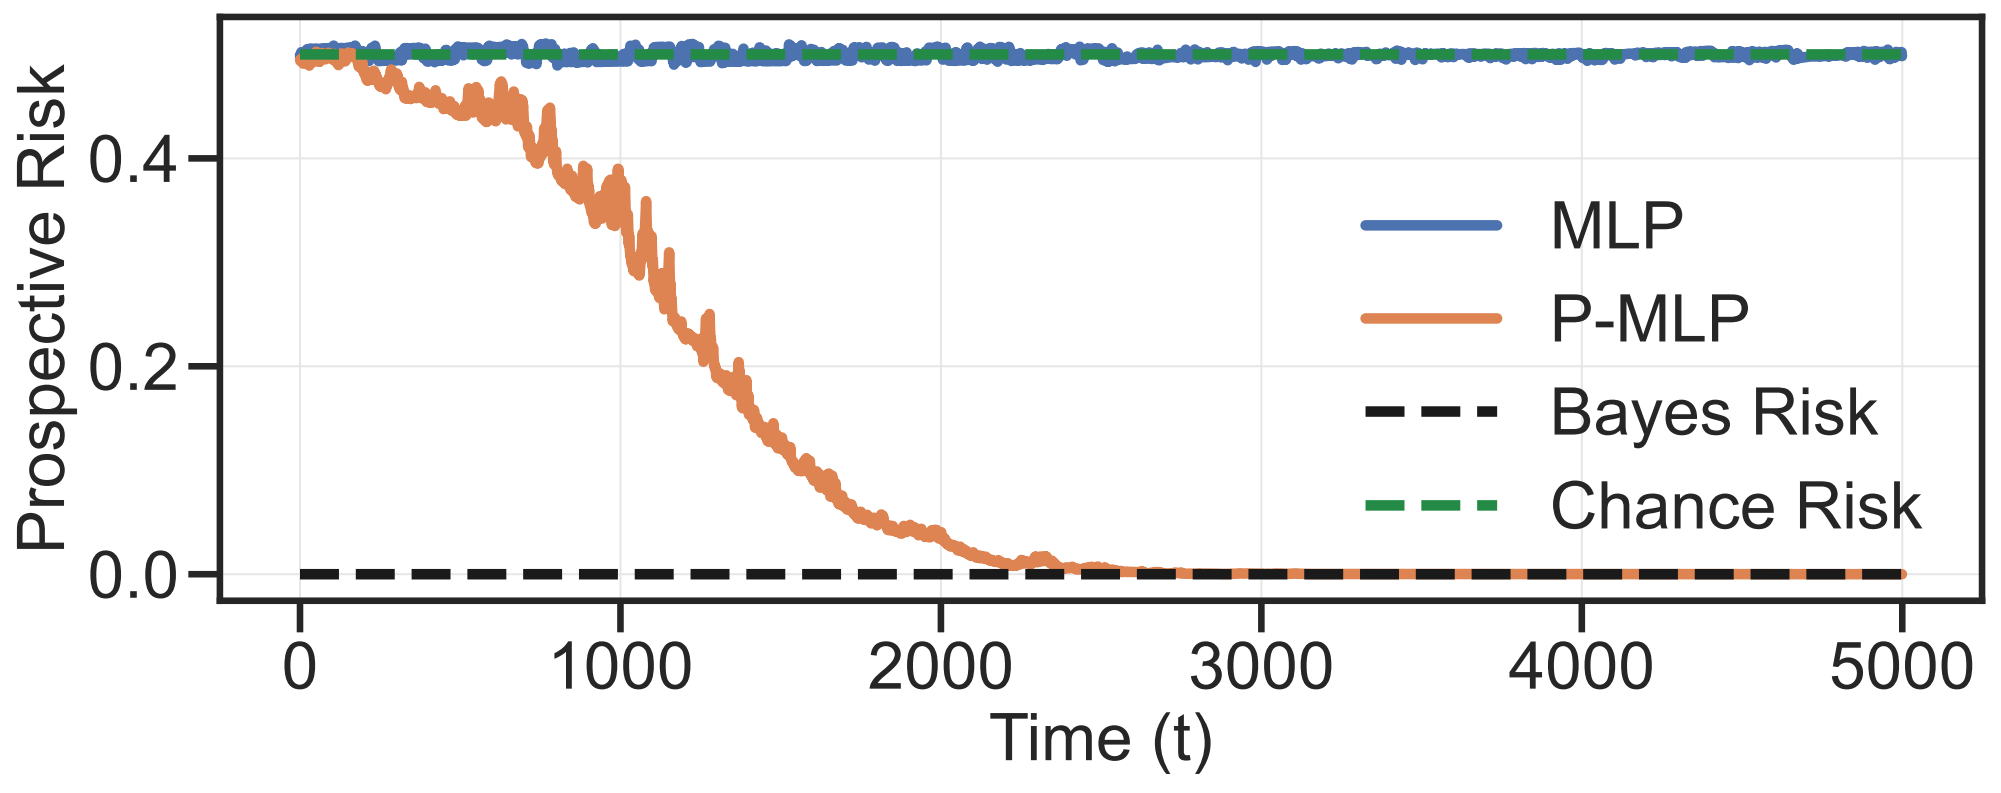
\includegraphics[width=\textwidth]{AGI5.png}
        \caption{长期学习中的预期风险趋势}
        \label{fig:agi_long_term_risk}
    \end{subfigure}
    \hfill
    \begin{subfigure}[b]{0.49\textwidth}
        \centering
        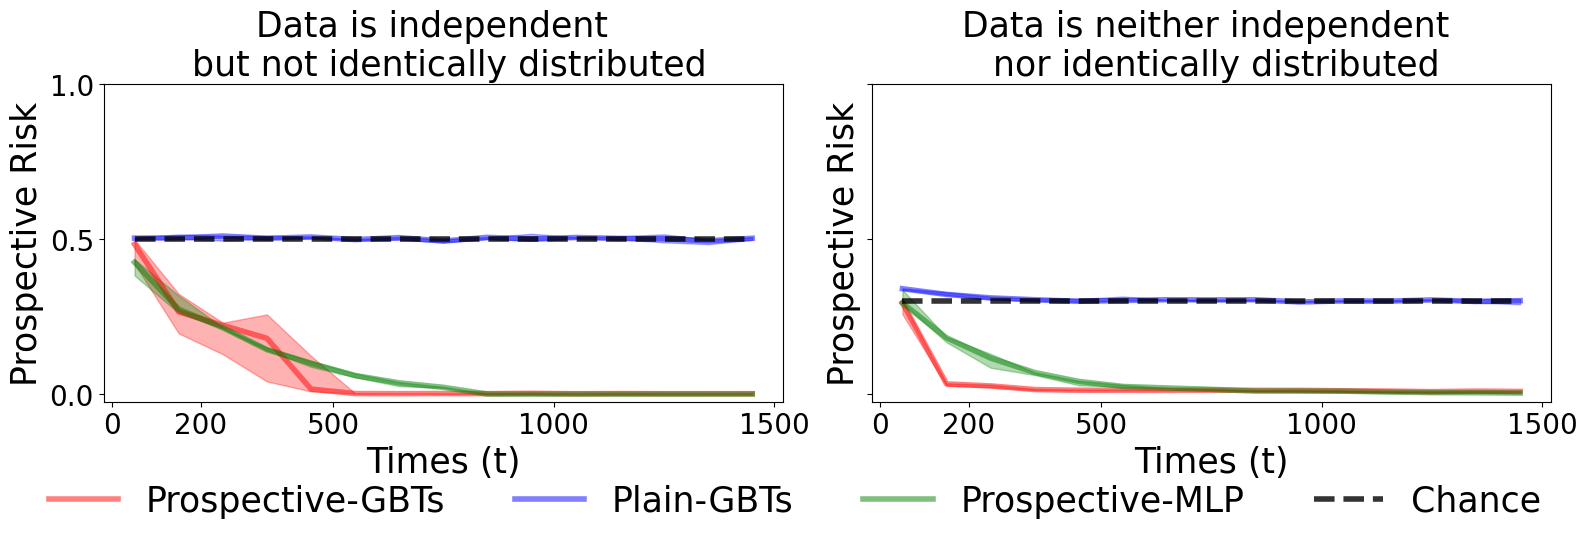
\includegraphics[width=\textwidth]{AGI9.png}
        \caption{非独立同分布数据下的预期风险}
        \label{fig:agi_non_iid_risk}
    \end{subfigure}
    \caption{通用智能体在复杂数据条件下的学习与风险控制。左图展示了MLP和P-MLP模型在长时间学习过程中预期风险的变化,突出P-MLP在持续学习和风险降低方面的优势。右图进一步探讨了当数据不满足独立同分布(IID)假设时,不同算法(Prospective-GBDTs, Plain-GBDTs, Prospective-MLP)的预期风险,强调AGI处理真实世界复杂数据时的必要性。}
    \label{fig:agi_complex_data_learning}
\end{figure}

为了量化AGI在通用能力上的突破,研究者们提出了“Jolt Analysis”,旨在识别性能曲线中显著的、非线性的跳跃,这可能预示着模型涌现出新的能力。

\begin{figure}[H]
    \centering
    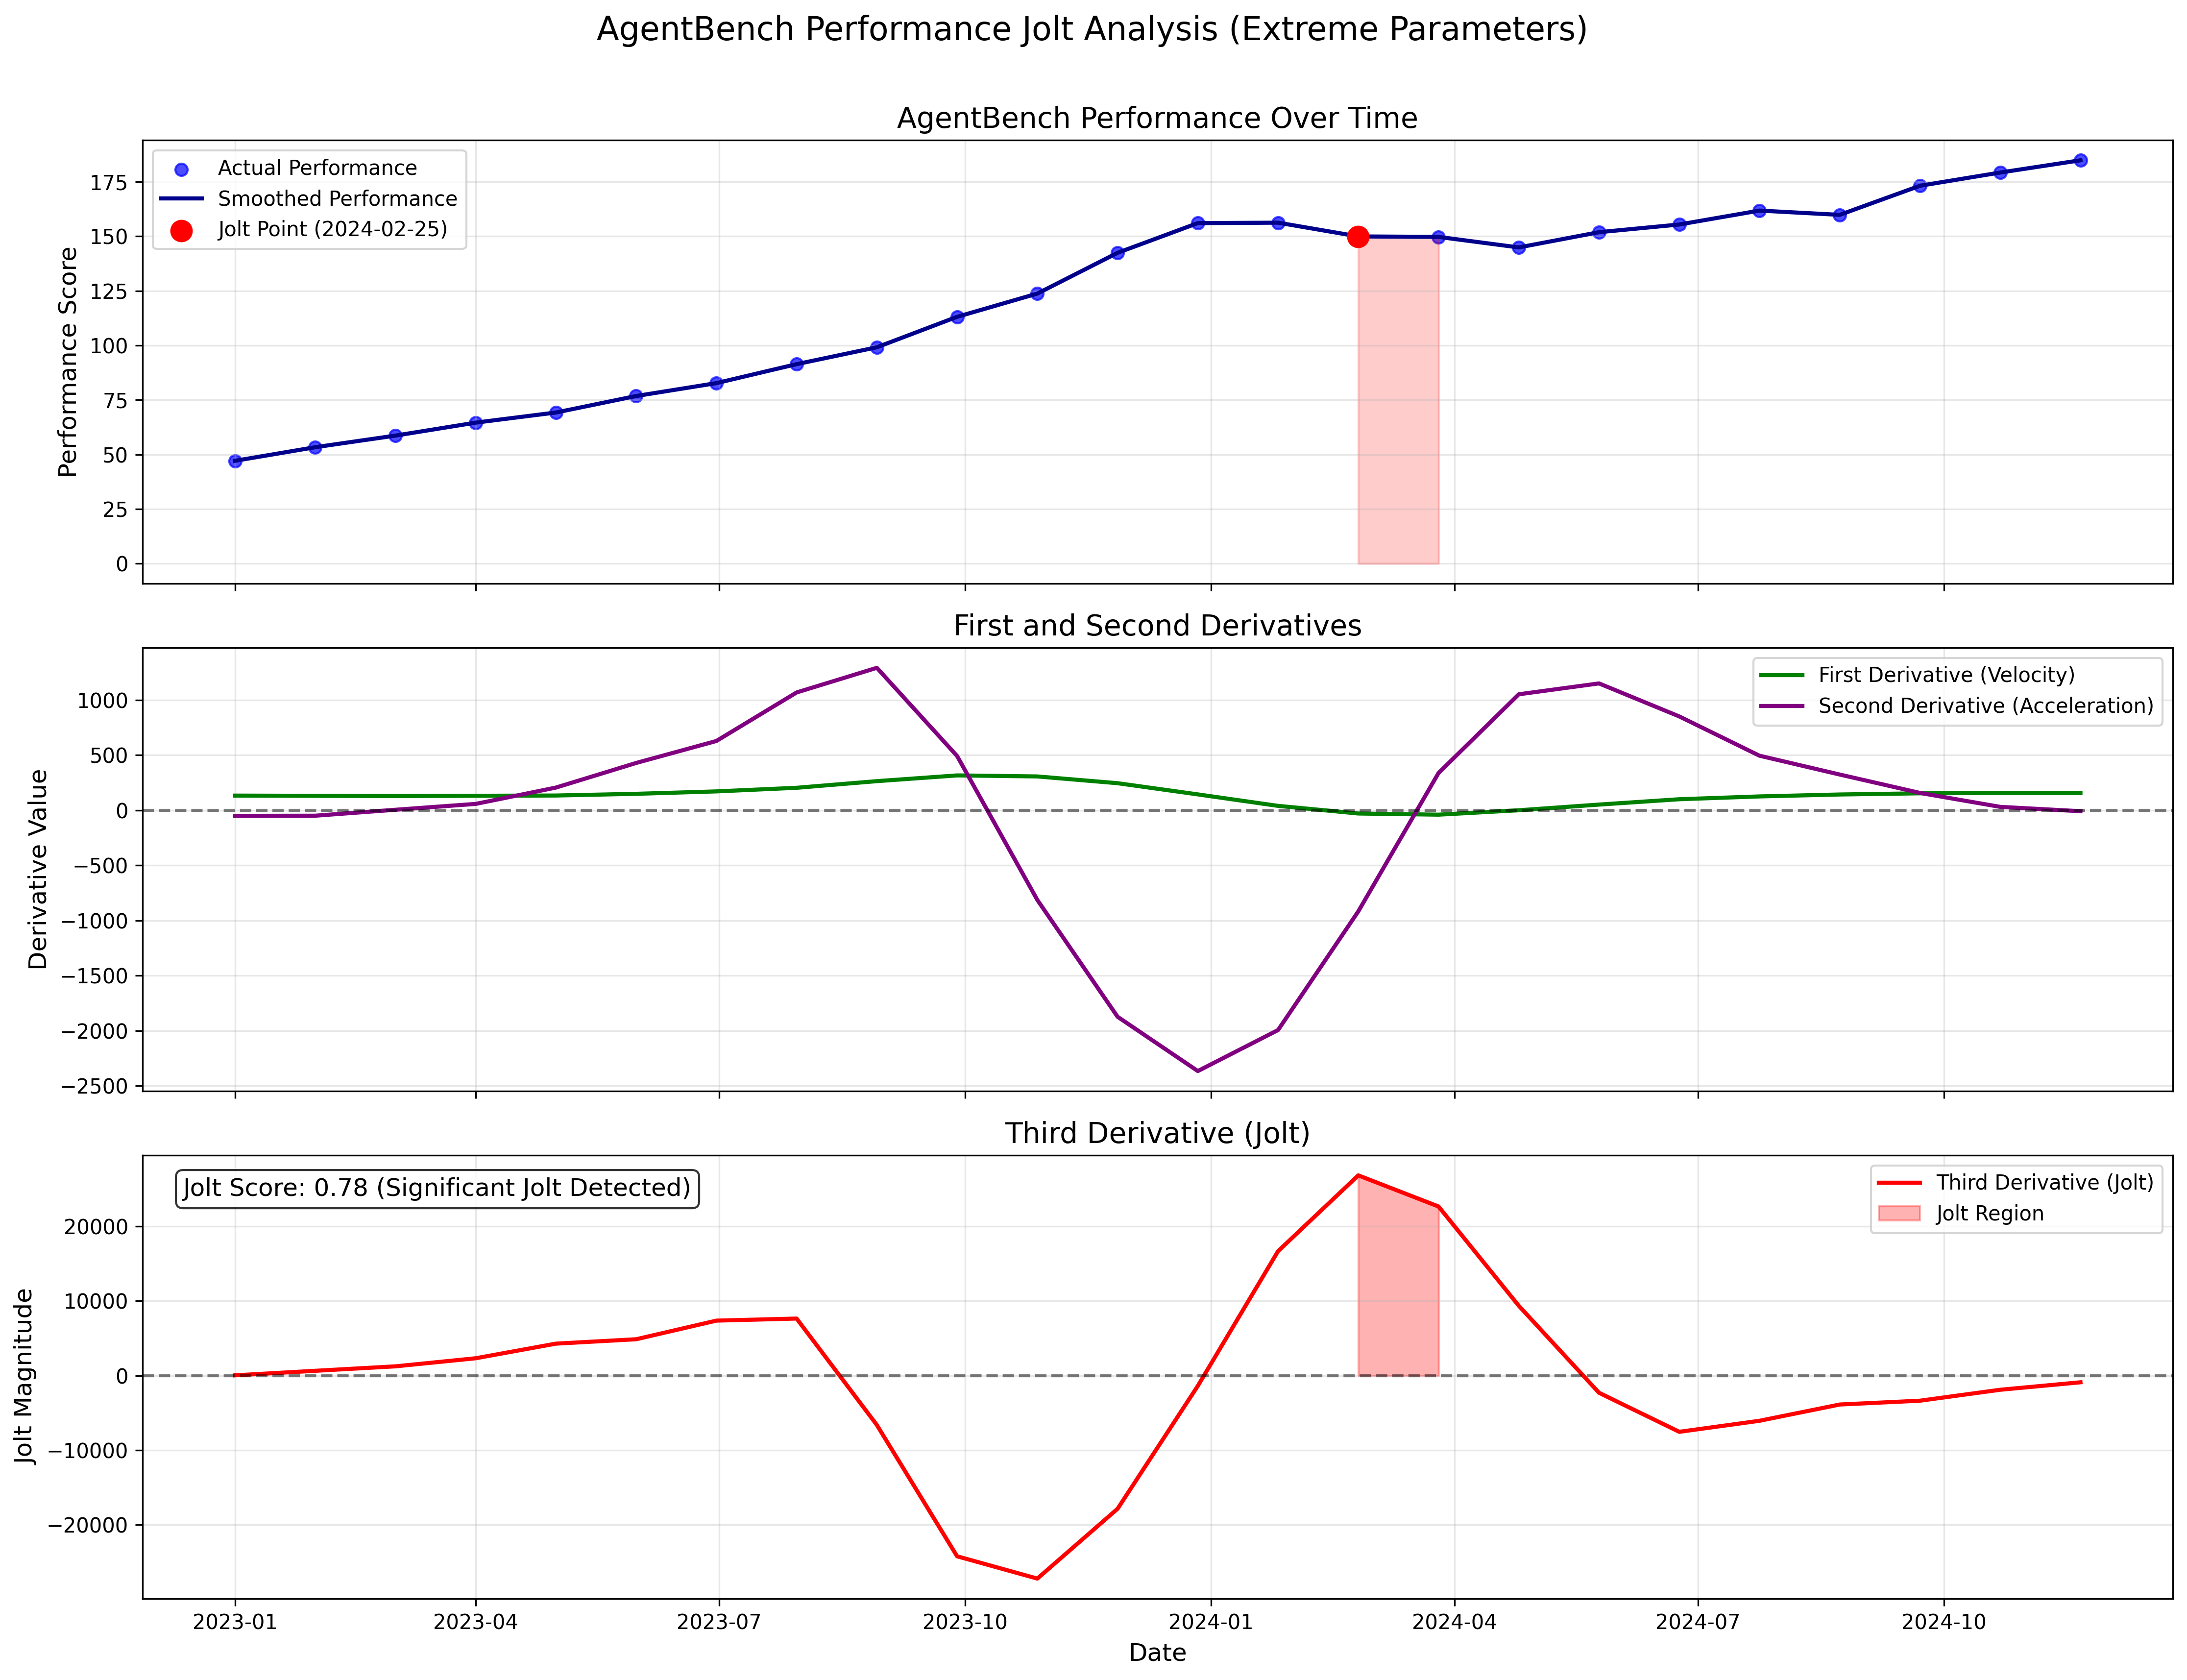
\includegraphics[width=0.9\textwidth]{AGI10.png}
    \caption{AgentBench性能的Jolt分析}
    \label{fig:agi_jolt_analysis}
\end{figure}
图 \ref{fig:agi_jolt_analysis} 展示了AgentBench性能随时间的变化,并对其一阶、二阶、三阶导数(Jolt)进行分析,以识别性能上的“显著跳跃”或“涌现点”。这种分析方法旨在更精确地捕捉AGI发展中的非线性进展,而不是仅仅依赖于平均性能的线性提升。

AGI的最终目标可以概念化为一个通用优化问题,它不仅要最小化错误,还要最大化知识获取和泛化能力。我们可以设想一个通用的学习目标函数,它旨在在多种任务和环境中实现最优表现:
$$
\mathcal{L}_{\text{AGI}}(\theta) = \sum_{i=1}^{M} \mathbb{E}_{x \sim \mathcal{D}_i} \left[ L(f_\theta(x), y_i(x)) \right] + \lambda_1 \mathcal{R}_{\text{knowledge}}(\theta) - \lambda_2 \mathcal{R}_{\text{complexity}}(\theta)
$$
其中,$M$ 是任务的数量,$\mathcal{D}_i$ 是第 $i$ 个任务的数据分布,$L$ 是损失函数,$f_\theta$ 是由参数 $\theta$ 定义的AGI模型,$\mathcal{R}_{\text{knowledge}}$ 是知识累积或泛化能力的正则项(目标是最大化),$\mathcal{R}_{\text{complexity}}$ 是模型复杂度的惩罚项(目标是最小化),$\lambda_1, \lambda_2$ 是权重系数。这个公式强调了AGI不仅要完成已知任务,还要不断学习、积累知识,并保持一定的效率和简洁性。

\subsection{人机协作的深化与人机共生社会}
未来,人与机器将更加紧密地协作,AI将成为人类的智能助手和增强工具。这种深化的人机协作将逐渐形成人机共生社会,共同推动社会进步。这种协作不仅仅是简单的工具使用,而是涉及知识共享、任务分配、共同决策和相互适应的复杂动态过程。

深化的人机协作体现在:
\begin{itemize}
    \item \textbf{增强人类智能:} AI系统将作为“认知助手”,帮助人类处理信息过载、进行复杂分析、提供决策支持,从而提升人类的创造力、生产力与解决问题的能力。例如,在医疗诊断、科学研究和金融分析中,AI可以快速处理大量数据并提供洞察。
    \item \textbf{智能自动化与互补:} AI将接管重复性、危险性或高精度的任务,解放人类去从事更具创造性、社交性或情感性的工作。人与机器将形成互补关系,各自发挥所长,共同完成复杂项目。例如,在工厂中,机器人处理物理劳动,而人类负责监督、编程和解决突发问题。
    \item \textbf{情感与社会互动:} 随着AI在自然语言处理、情感识别和生成方面的进步,未来的AI系统将能以更自然、更具同理心的方式与人类互动,例如在客户服务、教育辅导和老年护理等领域。
    \item \textbf{人机共学习:} 不仅仅是机器向人类学习,人类也将通过与AI系统的互动,学习新的知识和技能,甚至改变思维方式。
\end{itemize}

\subsection{人工智能在可持续发展目标中的作用}
AI有望在解决全球性挑战方面发挥关键作用,特别是在推动联合国可持续发展目标(SDGs)的实现上,其潜力巨大。

\begin{itemize}
    \item \textbf{气候变化:} AI可以助力应对气候变化,例如:
    \begin{itemize}
        \item \textbf{气候模型预测与优化:} 利用AI分析和融合多源气候数据,构建更精确的气候模型,预测极端天气事件和气候变化趋势,从而更好地规划应对策略。
        \item \textbf{能源系统优化:} 智能电网利用AI预测能源需求和可再生能源(如太阳能、风能)的波动性,优化电力分配,提高能源效率,减少对化石燃料的依赖。
        \item \textbf{碳排放监测与管理:} AI结合卫星图像和传感器数据,可以更精确地监测温室气体排放源,评估减排效果,并优化碳捕获与储存技术。
        \item \textbf{智慧农业:} 通过AI监控土壤健康、作物生长和水资源利用,实现精准农业,减少农药和化肥使用,降低农业碳足迹。
    \end{itemize}
    \item \textbf{能源优化:} AI能够优化能源生产、分配和消耗,提高能源利用效率。
    \begin{itemize}
        \item \textbf{建筑能源管理:} 智能建筑系统利用AI实时调节照明、暖通空调等,根据occupancy和天气预测优化能源消耗。
        \item \textbf{工业生产优化:} AI分析生产线数据,优化设备运行参数,减少能耗和废弃物,提升工业能效。
        \item \textbf{交通流量管理:} AI优化交通信号、路线规划和公共交通调度,减少交通拥堵,降低燃料消耗和排放。
    \end{itemize}
\end{itemize}

\subsection{对人类社会未来发展的深远影响与启示}
人工智能的发展将深刻重塑人类社会,从经济结构到文化生活都将受到影响,并引发对就业、道德、隐私和治理等方面的深刻反思。

\begin{itemize}
    \item \textbf{经济转型:} AI将推动产业升级和新经济模式的诞生,但也会加速传统行业的自动化,引发就业结构性变化。社会需要投资于劳动力再培训和终身学习,以适应新的人才需求。
    \item \textbf{文化与创意重塑:} AI在艺术、音乐、写作等领域的生成能力,将模糊人类与机器创作的界限,带来新的文化形式和伦理挑战。
    \item \textbf{社会治理与公平:} AI在公共服务、司法和政策制定中的应用,需要建立严格的伦理准则和监管框架,确保算法的公平性、透明度和可问责性,避免加剧社会不平等和偏见。
    \item \textbf{人类身份与价值:} 随着AI能力提升,人类将重新审视自身的独特价值,可能促使我们更关注创造力、批判性思维、情感智能和人际交往等非机械化能力。
    \item \textbf{全球合作与伦理共识:} AI技术的全球性影响要求各国加强国际合作,共同制定AI伦理规范、技术标准和法律框架,以确保AI的发展符合全人类的福祉和价值观。
\end{itemize}

我们需要以开放的心态拥抱AI带来的机遇,同时审慎应对其挑战,通过跨学科研究、政策创新和公众教育,构建一个负责任、可持续且普惠的人工智能生态系统,确保AI的发展能够真正造福全人类,构建一个更加智能、高效和可持续的未来。